%   Qualificação         = qualificacao 
%   Curso                = doutorado/mestrado
%   Situação do trabalho = pre-defesa/pos-defesa (exceto para qualificação)
% -- opções do pacote babel --
% Idioma padrão = brazil
	%spanish,			% idioma adicional para hifenização
	%english,			% idioma adicional para hifenização
	%brazil				% o último idioma é o principal do documento
\documentclass[doutorado, spanish, brazil, english]{packages/icmc}
\usepackage{rotating} 
\usepackage[all,knot,arc,import,poly]{xy}   
\usepackage{csvsimple}
\usepackage{tikz}
\usetikzlibrary{automata}
\usetikzlibrary{shapes.geometric, arrows}
\usetikzlibrary{mindmap,shadows}
\usepackage{booktabs}
\usetikzlibrary{fit, arrows, calc, positioning}
\newcommand{\VerbL}{0.52\textwidth}
\newcommand{\LatL}{0.42\textwidth}
\captionsetup{labelfont={color=red,bf},t,hangindent=0pt,textfont={color=black,bf}, format = plain}

% ---
% Informações de dados para CAPA e FOLHA DE ROSTO
% ---
\titulo{Development and enhancement of bioinformatic tools to integrate and understand aberrant epigenomic and genomic changes associated with cancer}
\autor[Silva, T. C.]{Tiago Chedraoui Silva}
\orientador[Orientador]{Prof. Dr.}{Houtan Noushmehr}
%\coorientador{Prof. Dr.}{Fulano de Tal}
\curso{ONCO}
\data{5}{8}{2017} % Data do depósito
% ---


% ---
% RESUMOS
% ---

% Resumo em português
% conter no máximo 500 palavras
\textoresumo[brazil]{

O câncer configura uma das maiores causas de mortalidade no mundo, caracterizando-se como uma doença complexa orquestrada por alterações genômicas e epigenômicas capazes de alterar a expressão gênica e a identidade celular. Nova evidência obtida por meio de um estudo genômico em larga escala e cujos dados encontram-se disponíveis no banco público do TCGA sugere que um em cada dez pacientes portadores de câncer pode ser classificado com maior eficácia tendo como base a taxonomia molecular quando comparada à histologia. Dessa maneira, nós hipotetizamos que o estabelecimento de mapas genômicos exibindo a localização de sítios de ligação de fatores de transcrição combinada à identificação de regiões diferencialmente metiladas e perfis alterados de expressão gênica possa nos auxiliar a caracterizar e explorar, ao nível molecular, fenótipos associados ao câncer.

Avanços tecnológicos e bancos de dados públicos a exemplo do The Cancer Genome Atlas (TCGA), The Encyclopedia of DNA Elements (ENCODE) e o NIH Roadmap Epigenomics Mapping Consortium (Roadmap) têm proporcionado um recurso inestimável para interrogar o (epi)genoma de linhagens de células tumorais em cultura, bem como de tecidos normais e tumorais em alta resolução. Todavia, a informação biológica encontra-se armazenada em diferentes formatos e não há ferramentas computacionais para integrar esses dados, evidenciando um cenário atual que requer, com urgência, o desenvolvimento de ferramentas de bioinformática e softwares capazes de direcionar a solução deste obstáculo.
Nesse contexto, o objetivo principal deste estudo consiste em implementar o desenvolvimento do pacote biOMICs, o qual será codificado usando-se a licença de código aberto GNU GPL e a linguagem de programação R e que, ao final do estudo, será submetido à comunidade científica do projeto Bioconductor. Além disso, ajudaremos nossos colaboradores com o aperfeiçoamento 
do ELMER, um pacote R/Bioconductor que  identifica elementos reguladores usando dados de expressão gênica, de metilação do DNA e análise de motivo.

Nossa expectativa é que o pacote biOMICs possa automatizar com acurácia a pesquisa, o download e a análise dos dados (epi)genômicos que se encontram atualmente disponíveis nas bases de dados públicas dos consórcios internacionais TCGA, ENCODE e Roadmap, além de integrá-los facilmente aos dados genômicos e epigenômicos gerados por pesquisadores por meio de experimentos em larga escala. Além disso, realizaremos também o processamento e a análise manual dos dados que serão automatizados pela ferramenta biOMICs, visando validar sua capacidade em descobrir assinaturas epigenômicas que possam redefinir subtipos de câncer. Por fim, usaremos biOMICs e ELMER para investigar as diferenças moleculares entre dois subgrupos de gliomas recentemente descobertos por nosso laboratório.}{Câncer, metilação do DNA, redes reguladoras de genes,  interações de cromatina, sitios de ligação do fator de transcrição, epi-genética, ferramentas computacionais}

% ---
% resumo em inglês
% ---
\textoresumo[english]{
Cancer, which is one of the major causes of mortality worldwide, is a complex disease orchestrated by aberrant genomic and epigenomic changes that can modify gene regulatory circuits and cellular identity. Emerging evidence obtained through high-throughput genomic data deposited within the public TCGA international consortium suggests that one in ten cancer patients would be more accurately classified by molecular taxonomy versus histology. Therefore, we have hypothesized that the establishment of genome-wide maps of the de novo DNA binding motifs localization coupled with differentially methylated regions and gene expression changes might help to characterize and exploit cancer phenotypes at the molecular level.

Technological advances and public databases like The Cancer Genome Atlas (TCGA), The Encyclopedia of DNA Elements (ENCODE), and The NIH Roadmap Epigenomics Mapping Consortium (roadmap) have provided unprecedented opportunities to interrogate the epigenome of cultured cancer cell lines as well as normal and tumor tissues with high resolution. Markedly however, biological information is stored in different formats and there is no current tool to integrate the data, highlighting an urgent need to develop bioinformatic tools and/or computational softwares to overcome this challenge. In this context, the main purpose of this study is the development of biOMICs, a package coded in the GNU GPL (General Public License) R programming language that will be submitted to the larger open-source Bioconductor community project. Also, we will help our collaborators improve of the R/Bioconductor ELMER package that identifies regulatory enhancers using gene expression, DNA methylation data and motif analysis.

Our expectation is that biOMICs can effectively automate search, retrieve, and analyze the vast (epi)genomic data currently available from TCGA, ENCODE, and Roadmap, and integrate genomics and epigenomics features with researchers own high-throughput data. Furthermore, we will also navigate through these data manually in order to validate the capacity of biOMICs in discovering epigenomic signatures able to redefine subtypes of cancer. Finally, we will use biOMICs and ELMER to investigate the molecular differences between two subgroups of gliomas, one of the most aggressive primary brain cancer, recently discovered by our laboratory.}{Cancer, DNA methylation, gene regulatory networks, enhancers, chromatin interactions, transcription factor binding sites, epi-genetics, computational tools}

% ---
% Configurações de aparência do PDF final
% ---
% alterando o aspecto da cor azul
\definecolor{blue}{RGB}{41,5,195}

% informações do PDF
\makeatletter
\hypersetup{
     	pagebackref=true,
		pdftitle={\@title}, 
		pdfauthor={\@author},
    	pdfsubject={\imprimirpreambulo},
	    pdfcreator={LaTeX with abnTeX2/FMRP-USP},
		pdfkeywords={\palavraschave}, 
		colorlinks=true,       		% false: boxed links; true: colored links
    	linkcolor=black,          	% color of internal links
    	citecolor=black,        		% color of links to bibliography
    	filecolor=black,      	% color of file links
		urlcolor=black,
		bookmarksdepth=4
}
\makeatother
% --- 

% ----------------------------------------------------------
% ELEMENTOS PRÉ-TEXTUAIS
% ----------------------------------------------------------

% Inserir a ficha catalográfica
%\incluifichacatalografica*{tex/fichaCatalografica.pdf}
\incluifichacatalografica{586} % Código Cutter: número atribuído ao sobrenome do autor. Para obtê-lo, consulte a tabela Cutter Sanborn (em http://203.241.185.12/asd/board/Author/upfile/abcd.htm), procure pelo sobrenome ou forma mais próxima ao sobrenome completo e coloque o número indicado como parâmetro.
\incluifolhadeaprovacao*{}

%\textofolha*{tex/pre-textual/folha-aprovacao}
% DEDICATÓRIA / AGRADECIMENTO / EPÍGRAFE
\textodedicatoria*{tex/pre-textual/dedicatoria}
\textoagradecimentos*{tex/pre-textual/agradecimentos}
\textoepigrafe*{tex/pre-textual/epigrafe}

% Inclui a lista de figuras
\incluilistadefiguras

% Inclui a lista de tabelas
\incluilistadetabelas

% Inclui a lista de quadros
\incluilistadequadros

% Inclui a lista de algoritmos
\incluilistadealgoritmos

% Inclui a lista de códigos
\incluilistadecodigos

% Inclui a lista de siglas e abreviaturas
\incluilistadesiglas

% Inclui a lista de símbolos
\incluilistadesimbolos

% ----
% Início do documento
% ----
\begin{document}
% ----------------------------------------------------------
% ELEMENTOS TEXTUAIS
% ----------------------------------------------------------
\textual

\chapter{Introduction}
\label{chapter:introducao}

\newcommand{\comando}[1]{\textbf{$\backslash$#1}}


\section{Objectives}

The main goal of this project is to develop tools for searching, retrieving and
analyzing pan-cancer genomic data from several databases, such as the NCI's
\sigla{GDC}{Genomic Data Commons}, which contains data from the \sigla{TCGA}{The Cancer Genome Atlas}
and \sigla{TARGET}{Therapeutically Applicable Research to Generate Effective Treatments},
\sigla{ENCODE}{The Encyclopedia of DNA Elements}, and
\sigla{ROADMAP}{The NIH Roadmap Epigenomics Mapping Consortium}.
For a better transparency, all tools will be open source and for their
scalability and interoperability they will be published in the Bioconductor project,
an environment that provides a broad range of powerful statistical and graphical methods
for the analysis of genomic data.
Furthermore, We also aim to investigate the intergenic epigenomic changes
associated with distinct biological and clinical subgroups of gliomas first
discovered by our laboratory \cite{ceccarelli2016molecular}. Specifically,
using the tools developed, we will integrate DNA methylation, gene expression,
mutation and copy number data as well as important epigenomic marks defined by
histone modifications in normal samples in order to identify candidate regulatory
elements associated with glioma progression.


\subsection{Specific aims}
\begin{enumerate}
    \item Download and process transcription factor (TF) ChIP-seq data for each cancer cell and tissue type through the ENCODE dataset;
    \item Download and process DNA methylation data for both cancer and non-tumor control cases through the TCGA consortium via HM450K platform;
    \item Identify statistically \sigla{DMR}{Differentially methylated regions} at the single CpG resolution;
    \item Determine statistically enriched proximal transcription factor binding sites (TFBSs) to altered DNA-methylated regions at the level of individual DNA/protein site interaction;
    \item Within known DMRs, classify and identify statistically known and novel DNA binding motifs;
    \item Download and process RNA-seq data from both cancer and non-tumor control cases;
    \item Use standard data structure to organize the data and the metadata;
    \item Correlate the DNA methylation status of \sigla{TFBSs}{Transcription factor binding sites} with target gene RNA-seq expression in order to determine regulatory networks that might alter the pan-cancer genome;
    \item Use learning machine algorithms for classifying an independent set of gliomas based on newly identified regulatory networks as related to pan-cancer deregulation;
    \item Develop tools to automate the previous steps;
    \item Use those tools to investigate the intergenic epigenomic changes associated with distinct biological and clinical subgroups of gliomas g-cimp-low and g-cimp-high discovered by our laboratory and collaborators;
    \item Compare the automated results with ones found manually in order to validate the package capacity in providing searching, retrieving and downstream biological analysis to discover pan-cancer epigenomic signatures able to redefine subgroups of gliomas;
    \item Submit those set of tools to be freely available in the open-source Bioconductor environment (available at \burl{http://www.bioconductor.org}).
\end{enumerate}

\section{Motivations}


Unravelling the genomic, epigenomic, and proteomic features using high-throughput methodologies is a central question for understanding regulatory gene networks in cancer. In this line of evidence, thousands of tumor and normal samples have been massively sequenced and a large amount of data are publicly deposited by the three main international consortia: TCGA, ENCODE, and Roadmap. However, a major challenge is the fact that the biological information necessary for a complete gene regulatory analysis is spread over different databases that store data in different formats. Moreover, to date there is a lack of  computational tools and methods that can integrate and interpret such information. Consequently, the process of analysis is performed manually by the end user, who must access all databases, select and process the data necessary to the project, and integrate that data using multiple downstream analysis tools to extract and interpret the relevant biological information.
To overcome these limitations, here we propose to implement tools for searching genomic and epigenomic data acquired from several biological databases, and to provide key scientific analysis steps and methodology, thereby allowing other researchers to apply  strategies for in-depth bioinformatics analysis. These tools will be submitted to Bioconductor, and then, our expectation is that researchers may integrate all relevant data from the most important international consortia in the genomics field with their own experiments. Providing our package through Bioconductor, enables us to access a broader scientific community of advanced informatics users and developers worldwide, who can test the package with their own microarray and next-generation sequencing data, submit bug reports, criticize the methodology, provide new contributions, and ensure the quality of our package in terms of code and documentation.  In addition, storing the outputs inside an open-source software like R, allows one to utilize the many available statistical and analytical packages commonly used by researchers \cite{creditcode}. Then, we expect that these tools will provide insights and novel discoveries into unanticipated regulatory circuits in complex disease and normal developmental biology, which will be verified through the molecular analysis between the newly identified groups G-CIMP-low and G-CIMP-high.


\section{Organization of the Remainder of the Document}

This paper is organized into chapters as follows: In Chapter 2,
fundamental concepts required to the development of this project are introduced.
We review the concepts of cancer and their epigenetic and genetic alterations,
followed by the description of the biological data generated through experiments
conducted to identify these changes and the data structure used to store it,
finally we reviewed some of the data analysis methods used in the genetics field.
Chapters 3, 4, and 5 highlights the results of this work. Specifically, in Chapter 3,
we detail the methods and computational tools developed, while in Chapter 4 we
show their application in the real world. Enclosing this thesis, in Chapter 5,
we draw the main conclusions of this work, as well as the scientific contributions
derived from this project, possible future works and the main papers
that have been published during the Doctorate period.


%\chapter{Instalando o abnTeX2}
%\label{chapter:instalando-abntex}
%A instalação do \emph{abnTeX2} varia de acordo com o sistema operacional empregado pelo usuário. Aqui serão apresentadas as formas de instalação nos sistemas mais utilizados atualmente, a saber: Linux (Ubuntu 12.04), Mac OS X e Windows 7

\section{Linux (Ubuntu 12.04)}

Se você já instalou o Tex Live via apt-get, basta seguir os seguintes comandos:

\begin{enumerate}

\item Baixe os arquivos de instalação do abnTeX2 (\url{http://code.google.com/p/abntex2/downloads/list}). Nesse link você também encontra a documentação e exemplos de uso.
\item Extraia o conteúdo do arquivo baixado na pasta texmf local, geralmente /usr/local/share/texmf. 
\item Em um Terminal: extraia o ZIP: \emph{unzip abntex2.tds.zip} em qualquer local;
\item copie o conteúdo extraído para o destino: \emph{cp abntex2/* /usr/local/share/texmf};
\item Em um Terminal digite: \emph{sudo texhash}
\item Pronto!
\end{enumerate}

\section{Mac OS}

Primeiramente, deve-se abrir o terminal do Mac que pode ser encontrado em Aplicativos/Utilitários - buscando pelo Finder.  E seguir os comandos abaixo:
\begin{enumerate}
\item Baixe os arquivos de instalação do abnTeX2 (\url{http://code.google.com/p/abntex2/downloads/list}). Nesse link você também encontra a documentação e exemplos de uso.
\item Extraia o conteúdo do arquivo baixado na pasta \emph{texmf} local, geralmente \emph{/usr/local/texlive/texmf-local}
\item Em um Terminal digite: \emph{sudo texhash}
\item Pronto!
\end{enumerate}
 
 \section{Windows 7}

\subsection{Instalar/atualizar pelo Package Manager (recomendado)}

Geralmente o abnTeX2 é baixado e instalado automaticamente pelo MiKTeX quando o usuário compila pela primeira vez um dos modelos do abnTeX2. Porém, caso isso não ocorra, siga os passos seguintes:

\begin{enumerate}
\item Clique em Iniciar/Start -> Todos os Programas/All Programs -> MiKTeX -> Package Manager;
\item Clique em Repository / Synchronize;
\item Clique com o botão direito sobre \emph{abntex2} na lista e selecione Install (ou Update, caso já esteja instalado);
\item Pronto!
\end{enumerate}

\subsection{Instalar/atualizar manualmente}

Você apenas precisará utilizar a instalação manual no caso de:

\begin{enumerate}
\item o abnTeX2 não estar na lista de pacotes do MiKTeX por alguma razão;
\item você não poder utilizar uma conexão com a Internet no momento da instalação;
\item a versão do abnTeX2 no MiKTeX estar desatualizada em relação à versão disponível no CTAN.
\end{enumerate}
Em qualquer caso, lembre-se de remover uma eventual instalação anterior do abnTeX2 . Se houver instalado pelo Package Manager, remova o abnTeX2 também por ele.

Passos para instalação manual do abnTeX2 no MiKTeX:

\begin{enumerate}
\item Baixe os arquivos de instalação do abnTeX2 (abntex2.tds-vX.X.zip). Nesse link você também encontra a documentação e exemplos de uso.
\item Extraia o conteúdo do arquivo baixado em uma pasta qualquer;
\item Você pode criar uma pasta abntex2, por exemplo, em $C:\backslash abntex2\backslash$;
\item Consulte http://www.tex.ac.uk/cgi-bin/texfaq2html?label=install-where para outras informações;
\item Clique em Iniciar/Start -> Todos os Programas/All Programs -> MiKTeX -> Settings;
\item Na aba Roots, adicione o diretório recém criado;
\item Na aba General, clique em Refresh FNDB, OU, se preferir, em um Terminal digite initexmf --update-fndb;
\item Pronto!
\end{enumerate}

%\chapter{Orientações gerais}
%\label{chapter:orientacoes-gerais}
%\section{Codificação dos arquivos: UTF8}

A codificação de todos os arquivos do pacote \abnTeX, incluindo a classe \textit{icmc}, é \texttt{UTF8}. É necessário que
você utilize a mesma codificação nos documentos que escrever, inclusive nos
arquivos de base bibliográficas |.bib|.



\section{Inclusão de outros arquivos}\label{sec-include}

É uma boa prática dividir o seu documento em diversos arquivos, e não
apenas escrever tudo em um único. Para tanto, esse recurso foi utilizado neste
documento, além de estarem organizados em um diretório separado do arquivo principal. Para incluir diferentes arquivos em um arquivo principal,
de modo que cada arquivo incluído fique em uma página diferente, utilize o
comando:

\begin{verbatim}
   \include{tex/documento-a-ser-incluido}      % sem a extensão .tex
\end{verbatim}

Para incluir documentos sem quebra de páginas, utilize:

\begin{verbatim}
   \input{tex/documento-a-ser-incluido}      % sem a extensão .tex
\end{verbatim}



\section{Remissões internas}

Ao nomear a \autoref{tab:lista_produtos} e a \autoref{fig:logomarca_usp}, apresentamos um exemplo de remissão interna, que também pode ser feita quando indicamos o \autoref{chapter:corpos-flutuantes}, que tem o nome \emph{\nameref{chapter:corpos-flutuantes}}. O número do capítulo indicado é \ref{chapter:corpos-flutuantes}, que se inicia à \autopageref{chapter:corpos-flutuantes}\footnote{O número da página de uma remissão pode ser obtida também assim:
\pageref{chapter:corpos-flutuantes}.}.

O código usado para produzir o texto desta seção é:

\begin{verbatim}
Ao nomear a \autoref{tab:lista_produtos} e a \autoref{fig:logomarca_usp}, apresentamos um exemplo de remissão interna, que também pode ser feita quando indicamos o \autoref{chapter:corpos-flutuantes}, que tem o nome \emph{\nameref{chapter:corpos-flutuantes}}. O número do capítulo indicado é \ref{chapter:corpos-flutuantes}, que se inicia à \autopageref{chapter:corpos-flutuantes}\footnote{O número da página de uma remissão pode ser obtida também assim: \pageref{chapter:corpos-flutuantes}.}.
\end{verbatim}

\section{Diferentes idiomas e hifenizações}
\label{sec-hifenizacao}

Para usar hifenizações de diferentes idiomas, inclua nas opções do documento o nome dos idiomas que o seu texto contém. Por exemplo (para melhor visualização, as opções foram quebras em diferentes linhas):

\begin{verbatim}
    \documentclass[
        qualificacao,
        mestrado
        pos-defesa,
        english,
        french,
        spanish,
        brazil
    ]{icmc}
\end{verbatim}

O idioma português-brasileiro (\texttt{brazil}) é incluído automaticamente pela classe \textsf{abntex2}. Porém, mesmo assim a opção \texttt{brazil} deve ser informada para que todos os pacotes reconheçam o idioma. Vale ressaltar que \textbf{a última opção de idioma é a utilizada por padrão} no documento. Desse modo, caso deseje escrever um texto em inglês que tenha citações em português e em francês, você deveria usar o preâmbulo como abaixo:

\begin{verbatim}
    \documentclass[
        doutorado,
        pre-defesa,
        french,
        brazil,
        english
    ]{icmc}
\end{verbatim}

A lista completa de idiomas suportados, bem como outras opções de hifenização, estão disponíveis em \citeonline[p.~5-6]{babel}.


\section{Comandos auxiliares úteis}

A classe \textit{icmc} contém alguns comandos auxiliares definidos com o objetivo de tornar o processo de escrita mais eficiente. Os principais comandos são apresentados a seguir:

\begin{description}
    
    \item[\comando{aspas\{CONTENT\}}] Comando utilizado para inserir um texto entre aspas.
    \item[\comando{autoref\{LABEL\}}] Comando utilizado para fazer referência a um elemento do texto. O parâmetro \texttt{LABEL} utilizado refere-se ao código definido por meio do comando \comando{label\{\}}.
    \item[\comando{fadaptada[CONTENT]\{REF\}}] Comando utilizado nos ambientes de \texttt{Figura}, \texttt{Tabela}, entre outros, para definir a origem da fonte do dado apresentado que foi adaptado de alguma referência. Os parâmetros utilizados são: \texttt{REF} que é o índice da referência no arquivo bibtex, e; \texttt{CONTENT} que é a localização exata do dado na referência (Ex.: p~30). O parâmetro \texttt{CONTENT} é opcional.
    \item[\comando{fautor}] Comando utilizado nos ambientes de \texttt{Figura}, \texttt{Tabela}, \texttt{Quadro}, entre outros, que define o próprio autor como provedor da informação.
    \item[\comando{fdadospesquisa}] Comando utilizado nos ambientes de \texttt{Figura}, \texttt{Tabela}, \texttt{Quadro}, entre outros, que define que os dados originaram da própria pesquisa.
    \item[\comando{fdireta[CONTENT]\{REF\}}] Comando utilizado nos ambientes de \texttt{Figura}, \texttt{Tabela}, \texttt{Quadro}, entre outros, para definir a origem da fonte do dado apresentado que foi adaptado de alguma referência. Os parâmetros utilizados são: \texttt{REF} que é o índice da referência no arquivo bibtex, e; \texttt{CONTENT} que é a localização exata do dado na referência (Ex.: p~30). O parâmetro \texttt{CONTENT} é opcional.
    \item[\comando{newword\{WORD\}\{DESC\}}] Comando utilizado para inserir palavras no glossário de modo mais prático. Os parâmetros utilizados são: \texttt{WORD} que é a palavra que será descrita, e; \texttt{DESC} que é o significado da palavra.
    \item[\comando{rev\{CONTENT\}}] Comando utilizado para inserir notas de revisão dentro do texto, as quais aparecerão destacadas em vermelho. O parâmetro utilizado é \texttt{CONTENT} que contém o texto sobre a revisão.
    \item[\comando{sigla\{ABBR\}\{DESC\}}] Comando utilizado para inserir siglas e abreviaturas na Lista de siglas de modo mais prático. Os parâmetros utilizados são: \texttt{ABBR} que é a abreviatura ou sigla, e \texttt{DESC} sua descrição. Ao utilizar esse comando, a sigla \textbf{também} é inserida no texto do documento.
    \item[\comando{sigla*\{ABBR\}\{DESC\}}] Comando utilizado para inserir siglas e abreviaturas na Lista de Siglas de modo mais prático. Os parâmetros utilizados são: \texttt{ABBR} que é a abreviatura ou sigla, e \texttt{DESC} sua descrição. Ao utilizar esse comando, a sigla é inserida \textbf{apenas} na Lista de Siglas.
    \item[\comando{simbolo\{SYM\}\{DESC\}}] Comando utilizado para inserir símbolos na Lista de Símbolos de modo mais prático. Os parâmetros utilizados são: \texttt{SYM} que é o símbolo, e \texttt{DESC} sua descrição. 
    
\end{description}


\section{Consulte o manual da classe \textsf{abntex2}}

Consulte o manual da classe \textsf{abntex2} \cite{abntex2classe} para uma
referência completa das macros e ambientes disponíveis. 

Além disso, o manual possui informações adicionais sobre as normas ABNT
observadas pelo \abnTeX\ e considerações sobre eventuais requisitos específicos, como o caso da \citeonline[seção 5.2.2]{NBR14724:2011}, que
especifica o espaçamento entre os capítulos e o início do texto.



\section{Precisa de ajuda?}

Consulte a FAQ com perguntas frequentes e comuns no portal do \abnTeX:
\url{https://code.google.com/p/abntex2/wiki/FAQ}.

Inscreva-se no grupo de usuários \LaTeX:
\url{http://groups.google.com/group/latex-br}, tire suas dúvidas e ajude
outros usuários.

Participe também do grupo de desenvolvedores do \abnTeX:
\url{http://groups.google.com/group/abntex2} e faça sua contribuição à
ferramenta.


\section{Você pode ajudar?}

Sua contribuição é muito importante! Você pode ajudar na divulgação,
desenvolvimento, aprimoramento e de várias outras formas. Veja como contribuir com a classe \textit{icmc} em
\url{https://github.com/lordantonelli/thesis-model-icmc} e faça sua contribuição.

%\chapter{Configuração dos elementos pré-textuais}
%\label{chapter:config-pre-textual}
%A configuração de diversas opções e principalmente dos elementos pré-textuais é realizada com comandos específicos inseridos antes do comando \comando{begin\{document\}}. As informações do documento são configuradas através dos comandos:

\begin{description}

 \item[\comando{titulo\{T\}}] Título do trabalho (substitua T pelo título do trabalho);

 \item[\comando{autor[REF]\{N\}}] Nome do autor do trabalho (onde REF é como o nome do autor é referenciado e N é o nome do autor);

 \item[\comando{orientador\{T\}\{O\}}] Nome do professor orientador do trabalho. Caso seja uma orientadora pode ser usado o comando \comando{orientador[Orientadora]\{T\}\{O\}} (sendo que T é a titulação do professor e O é o nome do orientador);

 \item[\comando{coorientador\{T\}\{C\}}] Nome do professor coorientador do trabalho. Caso seja uma coorientadora pode ser usado um comando análogo a definição de orientadora  empregando o comando \comando{coorientador[Coorientadora]\{T\}\{C\}}(sendo que T é a titulação do professor e C é o nome do orientador);

 
 \item[\comando{curso\{SPPG\}}] Dados do programa de Pós-Graduação, onde SPPG é a sigla do programa de pós-graduação. Exemplo: \comando{curso\{CCMC\}}. Os seguintes programas de Pós-Graduação estão disponíveis e configurados neste \textit{template}:
    \begin{itemize}
        \item \textbf{CCMC} -- Programa de Pós-Graduação em Ciências de Computação e Matemática Computacional
        \item \textbf{MAT} -- Programa de Pós-Graduação em Matemática
        \item \textbf{PIPGES} -- Programa Interinstitucional de Pós-Graduação em Estatística
        \item \textbf{PROFMAT} -- Programa de Pós-Graduação em Mestrado Profissional em Matemática em Rede Nacional
        \item \textbf{MECAI} -- Programa de Pós-Graduação em Mestrado Profissional em Matemática, Estatística e Computação Aplicadas à Indústria
    \end{itemize}
 
 \item[\comando{data\{dia\}\{mês\}\{ano\}}] Configuração da data do depósito do documento;

 \item[\comando{textoresumo\{TR\}\{PC\}}] Texto do resumo (TR) e palavras-chave (PC) do documento sendo separadas por vírgula. Se o idioma do resumo for diferente do declarado no documento, pode ser usado o comando \comando{textoresumo[L]\{TR\}\{PC\}} (sendo que L é a linguagem do resumo);
 
 \item[\comando{incluifichacatalografica\{COD\}}] Ficha catalográfica do documento gerada automaticamente de acordo com as informações do próprio documento mediante o fornecimento do código Cutter (COD). O \textbf{Código Cutter} é um número atribuído ao sobrenome do autor. Para obtê-lo, consulte a tabela Cutter Sanborn (em \url{http://www.davignon.qc.ca/cutter1.html}), procure pelo sobrenome ou forma mais próxima ao sobrenome completo e coloque o número indicado como parâmetro. Outra alternativa é gerar a ficha catalográfica diretamente no site da biblioteca \url{http://www.icmc.usp.br/Portal/Sistemas/Biblioteca/ficha.php} e inserir o PDF gerado por meio do comando \comando{incluifichacatalografica*\{ARQ\}}, em que ARQ é o nome do arquivo, incluindo o caminho do diretório se necessário.

 
\end{description}

As opções seguintes correspondem também as configurações dos elementos pré-textuais, porém seu uso é opcional: 

\begin{description}

 \item[\comando{textodedicatoria\{TD\}}] Texto referente a dedicatória do trabalho (TD). Caso o texto esteja em um arquivo separado (recomendado para que o projeto fique modularizado e os documentos mais limpo), deve utilizar o comando \comando{textodedicatoria*\{ARQ\}}, em que ARQ é o nome do arquivo, incluindo o caminho do diretório se necessário;

 \item[\comando{textoagradecimentos\{TA\}}] Texto referente aos agradecimentos do trabalho (TA). Caso o texto esteja em um arquivo separado (recomendado para que o projeto fique modularizado e os documentos mais limpo), deve utilizar o comando \comando{textoagradecimentos*\{ARQ\}}, em que ARQ é o nome do arquivo, incluindo o caminho do diretório se necessário;

 \item[\comando{incluilistadefiguras}] Comando para inclusão da lista de figuras. Deve-se utilizar este comando somente quando o ambiente \textbf{figure} for utilizado no documento;
 
 \item[\comando{incluilistadetabelas}] Comando para inclusão da lista de tabelas. Deve-se utilizar este comando somente quando o ambiente \textbf{table} for utilizado no documento;
  
 \item[\comando{incluilistadequadros}] Comando para inclusão da lista de quadros. Deve-se utilizar este comando somente quando o ambiente \textbf{quadro} for utilizado no documento;
   
 \item[\comando{incluilistadealgoritmos}] Comando para inclusão da lista de algoritmos. Deve-se utilizar este comando somente quando o ambiente \textbf{algoritmo} for utilizado no documento;
    
 \item[\comando{incluilistadecodigos}] Comando para inclusão da lista de figuras. Deve-se utilizar este comando somente quando o ambiente \textbf{codigo} for utilizado no documento;
 
 \item[\comando{incluilistadesiglas}] Comando para inclusão da lista de siglas e abreviaturas. Deve-se utilizar este comando somente quando existirem siglas e abreviaturas no documento, com a utilização do comando \comando{sigla\{S\}\{DS\}} ou \comando{sigla*\{S\}\{DS\}};

 \item[\comando{incluilistadesimbolos}] Comando para inclusão da lista de símbolos. Deve-se utilizar este comando somente quando existirem símbolos no documento, com a utilização do comando \comando{simbolo\{S\}\{DS\}}.
 
\end{description}

%\chapter{Corpos flutuantes}
%\label{chapter:corpos-flutuantes}
%Corpos flutuantes são elementos não textuais, como figuras e tabelas, que complementam as informações do texto. Neste capítulo são expostos breves exemplos dos corpos flutuantes disponíveis na classe \textit{icmc}.

Na \autoref{secao:figuras} é mostrado como inserir figuras, a \autoref{secao:tabelas_e_quadros} explica como incluir tabelas e quadros, a \autoref{secao:algoritmos_e_codigos} demostra como trabalhar com algoritmos e códigos-fonte e a \autoref{secao:outros-ambientes} explica como definir outros ambientes para serem utilizados, como para gráficos e diagramas.

\section{Figuras}
\label{secao:figuras}

A inserção de figuras é realizada normalmente através do comando \comando{begin\{figure\}}. Na \autoref{fig:logomarca_usp} é exibida a logomarca da USP com o pacote \textit{graphicx}. Já a \autoref{figura:exemplo_grafo} mostra um exemplo de grafo com o pacote \textit{xy}. De acordo com as normas ABNT a lista de figuras é um elemento opcional do documento, para incluí-la é preciso inserir o comando \comando{incluidelistafiguras} antes do início do documento.

Observe que, segundo a \citeonline[seções 4.2.1.10 e 5.8]{NBR14724:2011}, as
ilustrações devem sempre ter numeração contínua e única em todo o documento. Além disso, deve ser incorporado ao corpo flutuante do tipo figura, além da legenda, a fonte de onde esta foi extraída. Se a figura foi confeccionada pelo próprio autor, deve se colocar "Elaborada pelo autor".

\begin{citacao}
Qualquer que seja o tipo de ilustração, sua identificação aparece na parte
superior, precedida da palavra designativa (desenho, esquema, fluxograma,
fotografia, gráfico, mapa, organograma, planta, quadro, retrato, figura,
imagem, entre outros), seguida de seu número de ordem de ocorrência no texto,
em algarismos arábicos, travessão e do respectivo título. Após a ilustração, na
parte inferior, indicar a fonte consultada (elemento obrigatório, mesmo que
seja produção do próprio autor), legenda, notas e outras informações
necessárias à sua compreensão (se houver). A ilustração deve ser citada no
texto e inserida o mais próximo possível do trecho a que se
refere. \cite[seções 5.8]{NBR14724:2011}
\end{citacao}

\begin{figure}[htb]
 \caption{Logomarca da USP}
 \label{fig:logomarca_usp}
 \centering
 
\includegraphics[scale=0.3]{usp-logo.pdf}
 \fdireta{usp:logo}
\end{figure}


\begin{figure}[htb]
\caption{Exemplo de grafo}
\label{figura:exemplo_grafo}
\centering
\begin{scriptsize}
$$
\xymatrix@R20pt@C10pt{
 & & & & vr \ar[dlll] \ar[dl] \ar[d] \ar[dr] \ar[drr] \ar[drrr] & & & \\
 & (a_3, b_2, c_1) \ar[d]^{\varphi_2} \ar[dl]_{\varphi_1} & & (a_3, b_2, c_2) \ar[d]^{\varphi_2} \ar[dl]_{\varphi_1} & (a_1, b_1, c_1) & (a_1, b_1, c_2) & (a_1, b_2, c_1) & (a_1, b_2, c_2) \\
 (a_2, b_2, c_1) \ar[dr]_{\varphi_3} & (a_3, b_1, c_1) \ar[d]^{\varphi_1} & (a_2, b_2, c_2) \ar[dr]_{\varphi_3} & (a_3, b_1, c_2) \ar[d]^{\varphi_1} & & & & \\
& (a_2, b_1, c_1)  & & (a_2, b_1, c_2) & & & & \\
}
$$
\end{scriptsize}
\fautor
\end{figure}

A classe \textit{icmc} traz algum comando que auxiliam na inserção da legenda, para utilizá-los basta substituir o \comando{fonte\{\}} por um dos seguintes comando conforme necessário:

\begin{description}

 \item[\comando{fautor}] Insere o texto \aspas{Elaborada pelo autor} como fonte da figura;

 \item[\comando{fadaptada[INF]\{REF\}}] Insere um texto informando que a figura foi adaptada de alguma referência bibliográfica (REF). INF refere-se ao local específico de onde a imagem foi extraída, como por exemplo o número da página. Além disso, INF é um parâmetro opcional e pode receber qualquer cadeia de texto;

 \item[\comando{fdireta[INF]\{REF\}}] Insere um texto informando que a figura próvem diretamente de alguma referência bibliográfica (REF). INF refere-se ao local específico de onde a imagem foi extraída, como por exemplo o número da página. Além disso, INF é um parâmetro opcional e pode receber qualquer cadeia de texto;
 
 \item[\comando{fdadospesquisa}] Insere o texto \aspas{Dados da pesquisa.} como fonte da figura;
 
\end{description}



\section{Tabelas e Quadros}
\label{secao:tabelas_e_quadros}

A inserção de tabelas e quadros é feita de forma semelhante a inserção de figuras, porém são utilizados os ambientes \textit{table} e \textit{quadro}. A principal diferença entre tabelas e quadros, de acordo com \citeonline{NBR14724:2011}, é que as tabelas são destinadas para informações numéricas e os quadros são mais adequados para informações textuais. Em geral, as tabelas devem estar padronizadas conforme o padrão do \citeonline{ibge1993} requerido pelas normas da ABNT para documentos técnicos e acadêmicos.

Como exemplos foram inseridas a \autoref{tab:lista_produtos} que exibe uma de lista de produtos (construída em \LaTeX) e a Tabela \autoref{tabela:populacao_america_sul} que mostra a população dos países da América do Sul (construída segundo o padrão do IBGE). Foi inserido também o \autoref{quadro:editores_texto_livres} com alguns editores que podem ser usados para se trabalhar com \LaTeX para demonstrar a inserção de quadros.

 A lista de tabelas também é um elemento opcional que pode ser incluída com o comando \comando{incluidelistatabelas} antes do início do documento. O mesmo acontece com a lista de quadros que pode ser incluída com o comando \comando{incluidelistaquadros}.

\begin{table}[htb]
\centering
\caption{Lista de produtos}
\label{tab:lista_produtos}
\begin{tabularx}{\textwidth}{X|l|r|r|r} \hline
Produto      & Unidade & Preço (R\$) & Quantidade & Total (R\$) \\ \hline
Arroz        & Kg      & 2,00        & 550        & 1.100,00    \\
Óleo de Soja & L       & 2,50        & 500        & 750,00      \\
Açucar       & Kg      & 3,00        & 100        & 300,00      \\ \hline
\end{tabularx}
\fdadospesquisa
\end{table}

\begin{table}[htb]
\IBGEtab{%
  \caption{População dos países da América do Sul} \label{tabela:populacao_america_sul}
}{%
\begin{tabular}{r|p{3cm}|r}        
\toprule
Código  & País            & População   \\ \midrule \midrule
1       & Brasil          & ~~~~~~191.480.630 \\ \midrule 
2       & Argentina       &  39.934.100 \\ \midrule 
3       & Colômbia        &  46.741.100 \\ \midrule 
4       & Paraguai        &   9.694.200 \\ \midrule 
5       & Uruguai         &   3.350.500 \\ \midrule 
6       & Peru            &  28.221.500 \\ \midrule 
7       & Equador         &  13.481.200 \\ \midrule 
8       & Bolívia         &   9.694.200 \\ \midrule 
9       & Venezuela       &  28.121.700 \\ \midrule 
10      & Chile           &  16.803.000 \\ \bottomrule
\end{tabular}
}{%
  \fdireta{wikipedia:2011:america_sul}%
  \nota{Esta é uma nota, que diz que os dados são baseados na
  regressão linear.}%
  \nota[Anotações]{Uma anotação adicional, que pode ser seguida de várias
  outras, porém são opcionais.}%
  }
\end{table}

\begin{quadro}[htb]
\caption{Editores de Texto Livres}
\label{quadro:editores_texto_livres}
\centering
\begin{tabular}{|l|l|r|}        \hline
Editor     & Multiplataforma & Específico para Latex \\ \hline
Kwriter    & Sim             & Não                   \\
Texmaker   & Sim             & Sim                   \\
Kile       & Sim             & Sim                   \\
Geany      & Sim             & Não                   \\ \hline
\end{tabular}
\end{quadro}

\section{Algoritmos e Códigos}
\label{secao:algoritmos_e_codigos}

Além dos corpos flutuantes convencionais para inserir figuras (\comando{begin\{figure\}}) e tabelas (\comando{begin\{table\}}), a classe \textit{icmc} possui mais dois tipos de corpos flutuantes um para algoritmos (\comando{begin\{algoritmo\}}) e outro para códigos-fonte (\comando{begin\{codigo\}}). A utilização de um ou de outro fica a critério do usuário. Como exemplo temos o \autoref{algoritmo:mdc1} que calcula o máximo divisor comum entre dois números e os Códigos-fonte \ref{codigo:notas_alunos} e \ref{codigo:metodo_leitura} que são uma consulta na \sigla{SQL}{\textit{Structured Query Language}} e uma sobrotina em \textit{Java}.

\begin{algoritmo}
\caption{Algoritmo para cálculo de máximo divisor comum MDC($n_1$,$n_2$)}
\label{algoritmo:mdc1}

 \KwIn{Dois números inteiros ($n_1, n_2$)}
 \If(\tcp*[f]{Garante que o maior número seja $n_1$}){$n_2 > n_1$}
   {troca valores de $n_1$ e $n_2$}
 \Repeat{$r > 0$}{
    $r \leftarrow$ resto da divisão de $n_1$ por $n_2$
    $n_1 \leftarrow n_2$
    $n_2 \leftarrow r$
 }
 \Return $n_1$
\end{algoritmo}

\begin{codigo}[caption = {Consulta SQL}, label={codigo:notas_alunos},language=SQL, breaklines=true]
SELECT a.nome_aluno AS aluno,
       d.nome_disciplina AS disciplina,
       m.nota AS nota
FROM aluno AS a,
     disciplina AS d,
     matriculado AS m
WHERE a.id_aluno = m.id_aluno
  AND d.id_disciplina = m.id_disciplina
ORDER BY a.nome_aluno, d.nome_disciplina;
\end{codigo}

\begin{codigo}[caption={Subrotina para obter uma entrada do usuário}, label={codigo:metodo_leitura}, language=Java, breaklines=true]
public static String Leitura(){
    BufferedReader reader = new BufferedReader(new InputStreamReader(System.in));
    try {
        return reader.readLine(); // Lê uma linha pelo teclado
    } catch (IOException e) {
        e.printStackTrace();
        return "";
    }
}
\end{codigo}

Existem diversos outros pacotes disponíveis para escrever algoritmos e códigos. Nos exemplos anteriormente foram utilizados o pacote \textit{algorithm} para definição do ambiente algoritmo e \textit{listings} para a definição do ambiente de código-fonte. O pacote \textit{algorithm} é usado para escrever algoritmos em alto nível \cite{janos:2005:algpseudocode}. Já o pacote \textit{listings} serve para escrever os códigos em diversas linguagens de programação \cite{moses:2006:listings}.

Caso sejam utilizados os ambientes de algoritmos e código podem ser incluídos os comandos \comando{incluidelistaalgoritmos} e \comando{incluidelistacodigos} antes do \comando{begin\{document\}} para que a lista de algoritmos e a lista de código sejam criadas.


\section{Ambientes Matemáticos}

A classe \textit{icmc} provê os seguintes ambientes matemáticos:
\begin{itemize}
 \item Teoremas (\comando{begin\{teorema\}[\ ]} ... \comando{begin\{teorema\}});
 \item Proposição (\comando{begin\{proposicao\}[\ ]} ... \comando{begin\{proposicao\}});
 \item Lema (\comando{begin\{lema\}[\ ]} ... \comando{begin\{lema\}});
 \item Corolário (\comando{begin\{corolario\}[\ ]} ... \comando{begin\{corolario\}});
 \item Exemplo (\comando{begin\{exemplo\}[\ ]} ... \comando{begin\{exemplo\}});
 \item Observação (\comando{begin\{observacao\}[\ ]} ... \comando{begin\{observacao\}});
 \item Definição (\comando{begin\{definicao\}[\ ]} ... \comando{begin\{definicao\}});
 \item demonstracao (\comando{begin\{demonstracao\}[\ ]} ... \comando{begin\{demonstracao\}}).
\end{itemize}

Abaixo temos um exemplo de proposição com sua demonstração:
\begin{proposicao}
 Sejam $a$ e $b$ reais, tais que $0<a<b$. Então $a^2<b^2$.
\end{proposicao}
\begin{demonstracao}
 Pela hipótese concluímos que $(b+a)>0$ e $(b-a)>0$.

Como $b^2-a^2=(b+a)(b-a)$ concluímos que $b^2-a^2>0$, ou seja, $a^2<b^2$.
\end{demonstracao}

Neste documento tratamos brevemente apenas dos ambientes mencionados anteriormente. Contudo, para escrever expressões matemáticas complexas é preciso estudar uma documentação mais específica como em \citeonline{cassagojr:1997:amslatex}.

Alguns dos ambientes matemáticos da classe \textit{icmc} podem ser usados também para outras finalidades como exemplos e definições.


\section{Definição de outros ambientes}
\label{secao:outros-ambientes}

O classe \textit{icmc} permite a criação de outros ambientes, além dos citados nas seções anteriores, caso seja necessário. Isso é possível graças a extensão da classe \textit{abntex}. O \autoref{codigo:novo-ambiente} deve ser inserido antes do início do documento para criação de um ambiente para gráficos. Para definição de outros ambientes, basta seguir o modelo.


\begin{codigo}[caption={Definição do ambiente \textbf{grafico}}, label={codigo:novo-ambiente}, language=Tex, breaklines=true]
\makeatletter

% Novo list of (listings) para GRÁFICOS --------------------------
\newcommand{\graficoname}{Gráfico}
\newcommand{\graficorefname}{Gráfico}
\newcommand{\listofgraficosname}{Lista de gráficos}

\addto\captionsenglish{% ingles
    %% adjusts names from abnTeX2
    \newcommand{\graficoname}{Graph}
    \newcommand{\graficorefname}{Graph}
    \newcommand{\listofgraficosname}{List of graphs}
}

\newfloat[chapter]{grafico}{logr}{\graficoname}
\newlistof{listofgraficos}{logr}{\listgraficoname}
\newlistentry{grafico}{logr}{0}

% configurações para atender às regras da ABNT
\renewcommand{\thegrafico}{\thechapter.\@arabic\c@grafico}
\setfloatadjustment{grafico}{\centering}
\renewcommand{\cftgraficoname}{\graficoname\space}
\renewcommand*{\cftgraficoaftersnum}{\hfill\textendash\hfill}
% ----------------------------------------------------------------

\makeatother
\end{codigo}

A utilização do novo ambiente no texto segue conforme o \autoref{codigo:usar-novo-ambiente}.

\begin{codigo}[caption={Como usar o ambiente \textbf{grafico}}, label={codigo:usar-novo-ambiente}, language=Tex, breaklines=true]
\begin{grafico}[htb]
\caption{Caption do gráfico}
\label{gra:modelo}
Este é o conteúdo do gráfico.
\end{grafico}
\end{codigo}

Comandos como \comando{autoref\{gra:modelo\}} funcionam normalmente.

Para imprimir a "Lista de gráficos" no documento, insira o \autoref{codigo:lista-novo-ambiente} na classe \textit{icmc}, de modo que ele seja impresso após a "Lista de ilustrações". O código deve ser inserido após a linha 1244.


\begin{codigo}[caption={Código para inserir lista de gráficos}, label={codigo:lista-novo-ambiente}, language=Tex, breaklines=true]
% ---
% inserir lista de gráficos
% ---
\pdfbookmark[0]{\listofgraficosname}{logr}
\listofgraficos*
\cleardoublepage
% ---
\end{codigo}

%\chapter{Listas}
%\label{chapter:listas}
%\section{Abreviaturas e Siglas}

A classe \textit{icmc} implementa a criação da lista de abreviaturas e siglas com o pacote \textit{nomencl}. A inserção de abreviaturas e siglas na lista é realizada com o comando \comando{sigla\{A\}\{B\}} que também insere o conteúdo da sigla no local do documento onde a mesma foi definida. Os parâmetros utilizados são: \textit{A} que é a sigla e \textit{B} que é o nome por extenso. Caso deseja-se inserir a sigla apenas na lista, pode-se utilizar o comando \comando{sigla*\{A\}\{B\}}.

Para se gerar a lista de siglas na parte pre-textual do documento é preciso incluir o comando \comando{incluidelistasiglas} antes do início do documento. Além disto, a compilação do documento deve conter o comando \textit{makeindex} após duas compilações com o \textit{pdflatex}. Por exemplo, supondo que o documento principal tenha o nome de \textit{thesis}, podemos usar a seguinte sequência de comandos:

\begin{verbatim}
pdflatex thesis.tex
pdflatex thesis.tex
makeindex thesis.nlo -s nomencl.ist -o thesis.nls
pdflatex thesis.tex
\end{verbatim}

No \autoref{chapter:ferramentas-uteis} serão apresentadas algumas ferramentas que podem facilitar o processo de compilação do documento. Em especial, o ShareLaTeX não necessita de um processo de compilação especial para gerar a lista de abreviaturas e siglas.


\section{Símbolos}

A definição de símbolos é semelhante a definição de siglas, porém deve ser usado o comando \comando{simbolo\{S\}\{DS\}}, onde \textit{S} é o símbolo e \textit{DS} é a descrição do símbolo. Como exemplo definimos os símbolos $\mathbb{X}$\simbolo{\mathbb{X}}{Variável X} e $\mathsf{I\!R}$\simbolo{\mathsf{I\!R}}{Conjunto dos números reais}. Para incluir a lista de símbolos, basta usar o comando \comando{incluidelistasimbolos} antes do início do documento.

\chapter{Results}
\label{chapter:results}
%\input{tex/brca_analysis}


\section{Sotwares developed}

\section{ELMER}

Motivated by our discovery of transcriptional enhancers in tissue DNA methylation data \cite{berman2012ng}, and subsequent approaches to linking these enhancers to transcriptional targets using a chromQTL approach \cite{aran2013dna} (reviewed in \cite{yao2015review}), we developed the the R/Bioconductor  \textit{ELMER} (Enhancer Linking by Methylation/Expression Relationships) package, a tool which infers regulatory element landscapes and transcription factor networks from cancer methylomes \cite{yao2015inferring}. 

This tool combined DNA methylation and gene expression data from human tissues to infer multi-level cis-regulatory networks through several steps which included the identification of distal enhancer probes with significantly altered DNA methylation levels in primary tumor tissues compared to normal tissues, followed by the identification of putative target genes, and a comprehensive gene regulatory network analysis which combined transcription factor motifs at the altered enhancers with TF expression to identify the underlying master regulators. This approach identified several known and unknown master regulators in TCGA data, such as GATA3 and FOXA1 in breast cancer, and P63 and SOX2 in squamous cell lung carcinoma \cite{yao2015inferring,silva2016tcga}.

% Present \textit{ELMER}
Based on user feedback and a full review of the source code, we identified and implemented a number of software improvements, which are summarized in table \ref{tab:summary}: (i) The original package contained no standard data structure to handle multiple assays (DNA methylation, gene expression, and clinical data), which would be required for an integrative genomic data analysis. Recently, the Bioconductor team provided such a data structure through the \href{http://bioconductor.org/packages/MultiAssayExperiment/}{MultiAssayExperiment} package. (ii) All auxiliary databases (human TF list, classification of TF in families, gene annotation, DNA methylation annotation and motif occurrences within probe sites) used in the package were created and maintained manually, thereby making the upgrade process laborious; thus, we automated this process. (iii) The package was developed to analyze primary tumor tissue samples compared to normal tissues samples, thus not allowing arbitrary subgroups to be compared (for instance mutants vs. non-mutants, treated vs. untreated, etc.) (iv) Our original approach used known epigenomic markers for enhancers to constrain the genomic regions searched for differential methylation. However, this selection could limit our algorithm to identifying regulatory networks for tissue types that exist in the epigenomic databases; we found this constraint problematic, and thus now search \textit{all} distal regulatory regions without any such filter. (v) The function used to download data from The Cancer Genome Atlas (TCGA) data portal \cite{tomczak2015cancer} broke when the TCGA site was shutdown and its data transferred to The NCI's Genomic Data Commons (GDC) \cite{grossman2016toward}; we now have a more general data provider interface that supports GDC as the default provider. (vi) The package only supported data aligned to Genome Reference Consortium GRCh37 (hg19), and we now provide support for Genome Reference Consortium GRCh38 (hg38). (vii) There was no support to the recent HumanMethylationEPIC (EPIC) array \cite{epic}. In addition to the specific improvements listed above, we substantially re-wrote most of the code to be more efficient and maintainable,  also most of the output plots generated were improved.

\begin{table}[h!]
\centering
\caption{Main differences between ELMER old version (v.1) and the new version (v.2)}
\label{tab:summary}
\begin{tabular}{@{}p{3cm}p{5cm}p{6cm}@{}}
\toprule
\multicolumn{1}{c}{\textbf{Features}} & \multicolumn{1}{c}{\textbf{ELMER Version 1}} & \multicolumn{1}{c}{\textbf{ELMER Version 2}}   \\ \midrule
Primary data structure                   & mee object (custom data structure)                       & MAE object (Bioconductor data structure) \\
Auxiliary data                   & Manually created                       & Programmatically created \\
Number of human TFs                    & 1,982                                  & 1,987 (Uniprot database \cite{apweiler2004uniprot})                 \\
Number of TF motifs                   & 91                                     & 771  (HOCOMOCO v11 database \cite{kulakovskiy2016hocomoco})                 \\
TF classification                     & 78 families                            & 82 families and 331 subfamilies \newline(TFClass database \cite{wingender2013tfclass}) \\
Analysis performed            & Normal vs tumor samples & Group 1 vs group 2                       \\ 
Statistical grouping            & unsupervised only & unsupervised or supervised using labeled groups                       \\ 
TCGA data source                   & The Cancer Genome Atlas (TCGA) (not available)                   & The NCI's Genomic Data Commons (GDC)                                      \\
Genome of reference                   & GRCh37 (hg19)                          & GRCh37 (hg19)/GRCh38 (hg38)          \\
DNA methylation platforms             & HumanMethylation450                                   & HumanMethylationEPIC and HumanMethylation450                                \\
Graphical User interface (GUI)        & None                                   & TCGAbiolinksGUI                       \\
\bottomrule
\end{tabular}
\end{table}

Here, we present a new version of the R \textit{ELMER} package, which addresses all the issues described above. 
The new version of \textit{ELMER} (v2.0.0) is available as an R/Bioconductor package at \url{https://github.com/tiagochst/ELMER}. And, the new version of \textit{ELMER.data} (v2.0.0), which provides auxiliary data required to perform the analysis, is available at 
\url{https://github.com/tiagochst/ELMER.data}. 

\subsection*{Implementation}
% * <benbfly@gmail.com> 2017-06-09T18:49:35.529Z:
% 
% > Implementation
% Present and past tense are intermixed somewhat in this section.  I think we should use present tense for all methods descriptions, and only use past tense when we are describing a specific analysis run.
% 
% ^.
% For software tool papers, this section should address how the tool works and any relevant technical details required for implementation of the tool by other developers.  
Here we describe each of following analysis steps shown in figure \ref{fig:elmerworkflow}. For more details, please also check the original ELMER paper \cite{yao2015inferring}. 
\begin{itemize}
    \item Organize data as a \textit{MultiAssayExperiment} object
	\item Identify distal probes with significantly different DNA methylation level when comparing two sample groups.
	\item Identify putative target genes for differentially methylated distal probes, using methylation vs. expression correlation
	\item Identify enriched motifs for each probe belonging to a significant probe-gene pair
	\item Identify master regulatory Transcription Factors (TF) whose expression associate with DNA methylation changes at multiple regulatory regions.
\end{itemize}

Organization of data as a \textit{MultiAssayExperiment} object

To facilitate the analysis of experiments and studies with multiple samples the Bioconductor team created the \href{http://bioconductor.org/packages/SummarizedExperiment/}{\textit{SummarizedExperiment}} class \cite{huber2015orchestrating}, a data structure able to store data and metadata for a single experiment but not for data spanning several experiments for the same sample. To overcome this problem, recently, the MultiAssay SIG (Special Interest Group) created the \href{http://bioconductor.org/packages/MultiAssayExperiment/}{MultiAssayExperiment class} \cite{mae2017} a data structure to manage and preprocess multiple assays for integrated genomic analysis. This data structure is now an input for all main functions of \href{https://github.com/tiagochst/ELMER}{\textit{ELMER}} and can be generated by the \textit{createMAE} function. 

%In cancer research, integrative analysis of different molecular data associated with clinical outcome can be used to identify new subgroups of patients, which also might lead to specific improved therapy for this subset of patients \cite{kristensen2014principles}.
%With this trend of integrative analysis, the Bioconductor environment sought to provide a data structure that could integrate this data in the best possible way. One of those integrative data structures created was the \href{http://bioconductor.org/packages/SummarizedExperiment/}{\textit{SummarizedExperiment} container}, which was able to store several arrays if they have an equivalent number of rows and columns \cite{huber2015orchestrating}.


To perform \textit{ELMER} analyses, we need to populate a \textit{MultiAssayExperiment} with a DNA methylation matrix or \textit{SummarizedExperiment} object from HM450K or EPIC platform; a gene expression matrix or SummarizedExperiment object for the same samples; a matrix mapping DNA methylation samples to gene expression samples; and a matrix with sample metadata (i.e. clinical data, molecular subtype, etc.). If TCGA data are used, the last two matrices will be automatically generated.
If using non-TCGA data,  the matrix with sample metadata should be provided with at least a column with a patient identifier and another one identifying its group which will be used for analysis, if samples in the methylation and expression matrices are not ordered and with same names, a matrix mapping for each patient identifier their DNA methylation samples and their gene expression samples should be provided to the \textit{createMAE} function.
Based on the genome of reference selected, metadata for the DNA methylation probes, such as genomic coordinates, will be added from   \href{http://zwdzwd.github.io/InfiniumAnnotation}{\citeonline{zhou2016comprehensive}}; 
and metadata for gene expression and annotation is added from Ensembl database \cite{yates2015ensembl} using \href{http://bioconductor.org/packages/biomaRt/}{biomaRt}
\cite{durinck2009mapping}. 
% * <benbfly@gmail.com> 2017-06-08T12:50:39.539Z:
% 
% > the methylation and expression matrices of the {MultiAssayExperiment} can be populated using the \textit{XXXXXX} function
% @tiago can you fill this in?
% 
% ^ <tiagochst@gmail.com> 2017-06-09T21:44:31.369Z:
% 
% I'll try to rewrite this, actually the function is the same for TCGA and non-TCGA data, but the user will need to a the matrix mapping the samples to groups and another one to map gene expression to dna methylation columns if they don't have the same name. Also, gene expression rows needs to be ensembl gene id (ENSG).
%
% ^.

\subsubsection*{Selecting distal probes} 
Probes from HumanMethylationEPIC (EPIC) array and Infinium HumanMethylation450 (HM450) array are removed from the analysis if they have either internal SNPs close to the $3'$ end of the probe; non-unique mapping to the bisulfite-converted genome; or off-target hybridization due to partial overlap with non-unique elements \cite{doi:10.1093/nar/gkw967}. This probe metadata information is
included in \href{https://github.com/tiagochst/ELMER.data}{\textit{ELMER.data}} package, populated from the source file at \url{http://zwdzwd.github.io/InfiniumAnnotation} \cite{doi:10.1093/nar/gkw967}.
To limit ELMER to the analysis of distal elements, probes located in regions of $\pm2 kb$ around transcription start sites (TSSs) were removed.
% * <tiagochst@gmail.com> 2017-05-19T00:38:48.290Z:
% 
% > distal elements (not in promoter regions),
% Can we say this?
% 
% ^ <benbfly@gmail.com> 2017-06-08T12:55:23.253Z.

\subsubsection*{Identification of differentially methylated CpGs (DMCs)}

For each distal probe, samples of each group (group 1 and group 2) are ranked by their DNA methylation beta values, those samples in the lower quintile (20\% samples with the lowest methylation levels) of each group are used to identify if the probe is hypomethylated in group 1 compared to group 2, using an unpaired one-tailed t-test. The 20\% is a parameter to the \textit{diff.meth} function called \textit{minSubgroupFrac}. For the (ungrouped) cancer case, this is set to 20\% as in \citeonline{yao2015inferring}, because we typically wanted to be able to detect a specific molecular subtype among the tumor samples; these subtypes often make up only a minority of samples, and 20\% was chosen as a lower bound for the purposes of statistical power (high enough sample numbers to yield t-test p-values that could overcome multiple hypothesis corrections, yet low enough to be able to capture changes in individual molecular subtypes occurring in 20\% or more of the cases.) This number can be set arbitrarily as an input to the \textit{diff.meth} function and should be tuned based on sample sizes in individual studies. In the \textit{Supervised} mode, where the comparison groups are implicit in the sample set and labeled, the \textit{minSubgroupFrac} parameter is set to 100\%.  An example would be a cell culture experiment with 5 replicates of the untreated cell line, and another 5 replicates that include an experimental treatment.
% * <benbfly@gmail.com> 2017-06-08T13:32:21.874Z:
% 
% >  In the \textit{Supervised} mode
% I really would like to have a Supervised version of the pipeline where the percentage is not set at all, but automatically defaults to 100% .  This would be used for two group replicate comparisons like the one I describe.
% 
% ^ <tiagochst@gmail.com> 2017-06-09T21:47:56.390Z:
% 
% The pipeline you mean the TCGA_pipe function, which does all the code? We can remove percentage argument from it and add one "mode" supervised (all samples) unsupervised 20%. 
%
% ^ <tiagochst@gmail.com> 2017-06-09T23:50:55.816Z.
% * <benbfly@gmail.com> 2017-06-08T13:32:04.138Z:
% 
% > minSubgroupFrac
% What is the actual name of this parameter?  It should be named something intuitive since it is really important
% 
% ^ <tiagochst@gmail.com> 2017-06-09T21:48:57.068Z:
% 
% It was percentage in all functions. I'll see what I can do
%
% ^ <tiagochst@gmail.com> 2017-06-09T23:50:45.422Z:
% 
% I changed to minSubgroupFrac in the code
%
% ^ <tiagochst@gmail.com> 2017-06-09T23:50:51.139Z.

To identify hypomethylated DMCs, a one-tailed t-test is used to rule out the null hypothesis: $\mu_{group1} \geq \mu_{group2}$, where $\mu_{group1}$ is the mean methylation within the lowest group 1 quintile (or another percentile as specified by the \textit{minSubgroupFrac} parameter) and $\mu_{group2}$ is the mean within the lowest group 2 quintile. Raw p-values are adjusted for multiple hypothesis testing using the Benjamini-Hochberg method \cite{benjamini1995controlling}, and probes are selected when they had adjusted p-value less than $0.01$ (which can be configured using the \textit{pvalue} parameter). For additional stringency, probes are only selected if the methylation difference: $\Delta = \mu_{group1} - \mu_{group2}$ was greater than $0.3$. The same method is used to identify hypermethylated DMCs, except we use the \textit{upper} quintile, and the opposite tail in the t-test is chosen.
% * <benbfly@gmail.com> 2017-06-09T18:19:56.660Z:
% 
% > minDMCpval
% change this to the actual name
% 
% ^ <tiagochst@gmail.com> 2017-06-09T23:51:02.993Z.

\subsubsection*{Identification of putative target gene(s)} 

For each differentially methylated distal probe (DMC), the closest 10 upstream 
genes and the closest 10 downstream genes are tested for inverse correlation between 
methylation of the probe and expression of the gene (the number 10 can be changed using the \textit{numFlankingGenes} parameter). To select these genes, 
% * <benbfly@gmail.com> 2017-06-09T18:27:35.572Z:
% 
% > numFlankingGenes
% Does this parameter actually exist?  It should .. 
% 
% ^ <tiagochst@gmail.com> 2017-06-09T21:53:14.901Z:
% 
% I maintained Lijing's approach, we have a external function (https://github.com/tiagochst/ELMER/blob/master/R/GetNearbyGenes.R#L171-L176) . But I can change this and add to the get.pair and just add this numFlanking genes parameter.
%
% ^ <tiagochst@gmail.com> 2017-06-09T23:39:50.202Z:
% 
% I decided to keep the function outside. But I change the argument to numFlankingGenes instead of geneNum
%
% ^ <tiagochst@gmail.com> 2017-06-09T23:51:07.261Z.
the probe-gene distance is defined as the distance from the probe to the transcription 
start site specified by the ENSEMBL gene level annotations \cite{yates2015ensembl} accessed via
the R/Bioconductor package \href{http://bioconductor.org/packages/biomaRt/}{biomaRt} \cite{durinck2009mapping,durinck2005biomart}. By choosing a constant number of genes to test for each probe, our goal is to avoid systematic false positives for probes in gene rich regions. This is especially important given the highly non-uniform gene density of mammalian genomes.
Thus, exactly 20 statistical tests were performed for each probe, as follows. 

For each probe-gene pair, the samples (all samples from both groups) are divided into two 
groups: the M group, which consisted of the upper methylation quintile (the 20\%
of samples with the highest methylation at the enhancer probe), and the U group, 
which consists of the lowest methylation quintile (the 20\% of samples with the 
lowest methylation.) The 20\% ile cutoff is a configurable parameter \textit{minSubgroupFrac} in the \textit{get.pair} function.
As with its usage in the \textit{diff.meth} function, the default value of 20\% is a balance, allowing for the identification of changes in a 
molecular subtype making up a minority (i.e. 20\%) of cases, while also yielding 
enough statistical power to make strong predictions. For larger sample sizes or other experimental designs, this could be set even lower.

For each candidate probe-gene pair, 
the Mann-Whitney U test is used to test the null hypothesis that overall gene 
expression in group M is greater than or equal than that in group U. 
This non-parametric test was used in order to minimize the effects 
of expression outliers, which can  occur across a very wide dynamic range. 
For each probe-gene pair tested, the raw p-value $P_r$ is corrected for multiple 
hypothesis using a permutation approach as follows.
The gene in the pair is held constant, and \textit{x} random methylation probes are 
chosen to perform the same one-tailed U test, generating a set of \textit{x} permutation
p-values $P_p$. We chose the x random probes only from among those that were 
"distal" (farther than $2kb$ from an annotated transcription start site), in order 
to draw these null-model probes from the same set as the probe being tested \cite{sham2014statistical}. 
An empirical p-value $P_e$ value was calculated using the following formula 
(which introduces a pseudo-count of 1):

$$P_e = \frac{num(P_p \leq P_r)+ 1}{x+1}$$

Notice that in the \textit{Supervised} mode, no additional filtering is necessary to ensure that the M and U group segregate by sample group labels.  The two sample groups are segregated by definition, since these probes were selected for their differential methylation, with the same directionality, between the two groups. 



\subsubsection*{Characterization of chromatin state context of enriched probes using FunciVar}

Unlike version 1 of \textit{ELMER}, we now consider \textit{all} distal probes in the identification of regulatory elements. DNA methylation is known to affect several different classes of distal chromatin state element, including active enhancers, poised enhancers, and insulators. In order to provide a functional interpretation of the regulatory elements identified by \textit{ELMER}, we perform a chromatin state enrichment analysis of the probes within significant probe-gene pairs, using the \textit{statePaintR} tools from the \url{statehub.org} \cite{statepaintr}, along with our new FunciVar package \cite{funcivar}. Enrichment of the putative pairs within chromatin states is calculated against a background model that uses the distal probe set that the putative pairs are drawn from. 

\subsubsection*{Motif enrichment analysis}

In order to identify enriched motifs and potential upstream regulatory TFs, all probes with occurring in significant probe-gene pairs are combined for motif enrichment analysis. \sigla{HOMER}{Hypergeometric Optimization of Motif EnRichment} \cite{heinz2010simple} is used to find motif occurrences in a $\pm 250bp$ region around each probe, using \sigla{HOCOMOCO}{HOmo sapiens COmprehensive MOdel COllection} v11 \cite{kulakovskiy2016hocomoco} . Transcription factor (TF) binding models are available at \url{http://hocomoco.autosome.ru/downloads} (using the HOMER specific format with threshold score levels corresponding to p-value $ \leq 1^{-4}$). 

For each probe set tested (i.e. the set of all probes occurring in significant probe-gene pairs), a motif enrichment Odds Ratio and a 95\% confidence interval are calculated using following formulas:
$$p = \frac{a}{a + b}$$
$$P = \frac{c}{c + d}$$
$$Odds Ration = \frac{\frac{p}{(1-p)}}{\frac{P}{1-P}}= \frac{p(1-P)}{P(1-p)}=\frac{ad}{bc}$$
$$SD = \sqrt{\frac{1}{a} + \frac{1}{b} + \frac{1}{c} + \frac{1}{d}}$$

where $a$ is the number of probes within the selected probe set that contains one 
or more motif occurrences; $b$ is the number of probes within the selected probe 
set that do not contain a motif occurrence; $c$ and $d$ are the same counts within 
the entire array probe set (drawn from the same set of distal-only probes using the same definition as the primary analysis). A probe set was considered significantly enriched 
for a particular motif if the 95\% confidence interval of the Odds Ratio was 
greater than $1.1$ (specified by option \textit{lower.OR}, $1.1$ is default), and the motif 
occurred at least 10 times (specified by option \textit{min.incidence}, $10$ is default) in 
the probe set. 

%\section*{Results} % Optional - only if novel data or analyses are included
%This section is only required if the paper includes novel data or analyses, and should be written as a traditional results section.

\subsubsection*{Identification of master regulator TFs}

When a group of enhancers is coordinately altered in a specific sample subset, this is often the result of an altered upstream \textit{master regulator} transcription factor in the gene regulatory network. \textit{ELMER} tries to identify such transcription factors corresponding to each of the TF binding motifs enriched from the previous analysis step.
For each enriched motif, \textit{ELMER} takes the average DNA methylation of all distal probes (in significant probe-gene pairs) that contain that motif occurrence (within a $\pm 250bp$ region) and compares this average DNA methylation to the expression of each gene annotated as a human TF.

A statistical test is performed for each motif-TF pair, as follows. All samples 
are divided into two groups: the M group, which consists 
of the 20\% of samples with the highest average methylation at all motif-adjacent
probes, and the U group, which consisted of the 20\%  of samples with the lowest 
methylation. This step is performed by the \textit{get.TFs} function, which takes \textit{minSubgroupFrac} as an input parameter, again with a default of 20\%.
For each candidate motif-TF pair, the Mann-Whitney U test is used to test 
the null hypothesis that overall gene expression in group M is greater or equal 
than that in group U. This non-parametric test was used in order to minimize the 
effects of expression outliers, which can occur across a very wide dynamic range. 
For each motif tested, this results in a raw p-value ($P_r$) for each of the human TFs.
All TFs are ranked by their $-log_{10}(Pr)$ values, and those falling within the top 5\% of 
this ranking were considered candidate upstream regulators. The best upstream 
TFs which are known to recognize to specific binding motif are automatically extracted as putative 
regulatory TFs, and rank ordered plots are created to visually inspect these relationships, as shown in the example below. Because the same motif can be recognized by many transcription factors of the same binding domain family, we define these relationships at both the family and subfamily classification level using the 
classifications from TFClass database \cite{wingender2013tfclass}. Use of this database is a major change from version 1 of ELMER, which used custom curations for DNA binding domain families. Use of the TFClass database is preferable because it is well curated and regularly updated to reflect new findings.



%\begin{landscape}
\tikzstyle{container} = [
    rectangle,
    draw,
    inner sep=0.2 cm,
    dashed
]
\tikzstyle{start} = [circle,
					 minimum size=2mm,
                     rounded corners=3mm,
					 very thick,
                     draw=green!50!black,
                     top color=green!50!black,
                     bottom color=green!50!black, 
                     text=white,
                     font=\tiny]

\tikzstyle{end} = [circle,
				  minimum size=2mm,
                  rounded corners=3mm,
                  very thick,draw=red!50!black, 
                  top color=red!50!black,
                  bottom color=red!50!black, 
                  text=white,
                  font=\tiny]

\tikzstyle{function} = [rectangle,
						minimum size=6mm,
                        rounded corners=3mm,
                        very thick,
                        draw=black!50, 
                        top color=white,
                        bottom color=white,
                        font=\itshape\footnotesize]

\tikzstyle{datain} = [
	rectangle, 
	rounded corners, 
    minimum width=3cm, 
    minimum height=0.5cm,
    text centered,
    font=\footnotesize, 
    draw=green!50!black, 
    fill=white, 
    text=black
]
                      
\tikzstyle{dataaux} = [
	rectangle, 
    rounded corners, 
    minimum width=3cm, 
    minimum height=0.5cm,
    text centered,
    font=\footnotesize,
    draw=orange, 
    fill=white, 
    text=black
]
                       
\tikzstyle{dataout} = [
	rectangle, 
	rounded corners, 
    minimum width=3cm, 
    minimum height=0.5cm,
    text centered,
    font=\footnotesize, 
    draw=blue, 
    fill=white, 
    text=black
]

% Pacakge labels
\tikzstyle{arrow} = [
	thick,
    ->,
    >=stealth,
    -latex',
    draw,
    rounded corners
]

\tikzstyle{labelelmer}=[
	rectangle,
    draw,
    fill=black!50!red,
    draw = black,
    minimum width=450pt,
    minimum height=1.5em,
    text=white,
    rotate = 90, 
    label={[rotate=90]center:\textcolor{white}{\textbf{ELMER package}}}
]

\tikzstyle{labeltcgabiolinks}=[
	rectangle,
	draw,
    fill=black!50!blue,
    draw = black,
    minimum width=420pt,
    minimum height=1.5em,
    text = green,
    rotate = 90, 
    label={[rotate=270]center:\textcolor{white}{\textbf{TCGAbiolinks/TCGAbiolinksGUI packages}}}
]


\tikzstyle{labelfuncivar}=[
	rectangle,
	draw,
    fill=black!20!orange,
    draw = black,
    xshift = -0.0cm,
    minimum width=480pt,
    minimum height=1.5em,
    text=white,
    rotate = 0, 
    label={[rotate=0]center:\textcolor{white}{\textbf{StateHub/StatePaintR/funcivar package}}}
]
\tikzstyle{labelgdc}=[
	rectangle,
	draw,
    fill=black!50!gray,
    draw = black,
    minimum width=167pt,
    minimum height=1.5em,
    text=white,
    yshift = 0.10cm,
    xshift = 0.1cm,
    rotate = 0, 
    label={[rotate=0]center:\textcolor{white}{\textbf{GDC database}}}
]
\tikzstyle{every annotation}=[fill=white, font=\sf \small, scale=0.5, text width=4cm, inner sep=2mm, text=black,draw = orange]


\begin{figure}[!ht]
\centering
  \resizebox{0.95\textwidth}{!}{%
\begin{tikzpicture}[node distance = 1.5cm, auto, shorten >=1pt,thick,font=\itshape\footnotesize]
\linespread{0.8}{
%\node (start) [start] {START};
\node (func1) [function, yshift = -0.5cm] {\textit{createMAE}};
\node [datain, right of=func1, yshift = 0.5cm, xshift = 2cm] (dna) {DNA methylation object};
\node [datain, right of=func1, yshift = -0.5cm, xshift = 2cm] (exp) {Gene expression object};
\node (out1) [dataout, below of=func1, yshift = -0.3cm,text width=3cm] {Multi Assay Experiment object};
\node (func2) [function, below of = out1] {get.diff.meth};
%\node (out2) [dataout, below of=func2, yshift = 0.3cm] {List of differently methylated probes};
\node (func3) [function, below of=func2] {GetNearGenes};
%\node (out3) [dataout, below of=func2, yshift = 0.3cm] {List of near genes for differently methylated probes};
\node (func4) [function, below of=func3] {get.pair};
%\node (out4) [dataout, below of=func4, yshift = 0.3cm] {List of pairs: differently expressed gene and differently methylated probes};
\node (func5) [function, below of=func4, yshift = -0.5cm] {get.enriched.motif};
%\node (out5) [dataout, below of=func5, yshift = 0.3cm] {List of enriched motifs};
\node (func6) [function, below of=func5] {get.TFs};
\node (func7) [function, below of=func6,yshift = -0.5cm] {TF.survival};
%\node (out5) [dataout, below of=func5, yshift = 0.3cm] {List of regulator};
\node [dataaux, left of=func5, xshift =-3cm] (elmerdata1) {Probes.motif};
%\node [dataaux, above of=elmerdata1] (enhancer) {enhancer};
\node [dataaux, left of=func6, yshift = 0.0cm, xshift =-3cm] (elmerdata2) {motif.relevant.TFs};
\node [dataaux, left of=func6, yshift = -1.0cm, xshift =-3cm] (elmerdata3) {human.TFs};
%\node (end) [end, below of=func7] {END};
\node (func8) [function, left of=func1,yshift = -3cm,xshift = -3cm] {get.feature.probe};
\node (probes) [datain, left of=func1,xshift = -3cm] {distal probes};
\node [dataaux, below of=func8] (tss) {ENSEMBL TSS};
\node [dataaux, below of=tss] (probesmetadata) {Probes metadata};


% funcvat
\node (funciVar) [function, below of=func7, xshift = 3cm, yshift = -1.4cm] {enrich.segments};
\node [dataaux, left of=funciVar,xshift = -2cm] (statehub) {Statehub tracks};
%\node [dataaux, left of=statehub,xshift = -2cm, yshift = 0.2cm] (encode) {ENCODE};
%\node [dataaux, left of=statehub,xshift = -2cm, yshift = -0.4cm] (roadmap) {ROADMAP};
%\node [dataaux, left of=statehub,xshift = -2cm, yshift = 0.8cm] (blueprint) {BLUEPRINT};
%\draw [arrow,dashed,draw=orange] (encode.east) -- (statehub.west);
%\draw [arrow,dashed,draw=orange] (roadmap.east) -- (statehub.west);
%\draw [arrow,dashed,draw=orange] (blueprint.east) -- (statehub.west);

\draw [arrow,dashed,draw=orange] (statehub.east) -- (funciVar.west);

\draw [arrow] (func4) -- ++(4.9,0) -- ++(0,-1) |- node {} (funciVar);

% Draw edges
%\path [arrow] (start) -- (func1);
\path [arrow,dashed,draw=green!50!black] (dna) |- (func1);
\path [arrow,dashed,draw=green!50!black] (exp) |- (func1);
\draw [arrow,dashed,draw=blue] (out1.west) -- ++(-.5,0) -- ++(0,-1) |- (func4.west);
\draw [arrow,dashed,draw=blue] (out1.west) -- ++(-.5,0) -- ++(0,-1) |- (func6.west);
\draw [arrow] (func1) -- (out1);
\draw [arrow] (out1) -- (func2);
\draw [arrow] (func2) -- node {} (func3);
\draw [arrow] (func3) -- (func4);
\draw [arrow] (func4) -- node {} (func5);
\draw [arrow] (func5) -- node {}(func6);
\draw [arrow] (func6) -- (func7);
%\draw [arrow] (func7) -- (end);
\draw [arrow,dashed,draw=orange] (elmerdata1) -- node {} (func5);
\draw [arrow,dashed,draw=orange] (elmerdata2.east) -- (func6.west);
\draw [arrow,dashed,draw=orange] (elmerdata3.east) -- ++(.5,0) -- ++(0,0.2) |- (func6.west);
%\draw [arrow,dashed,draw=orange] (enhancer.north) -- (func8.south);
\draw [arrow,dashed,draw=orange] (tss.north) -- (func8.south);
\draw [arrow,dashed,draw=orange] (probesmetadata.east) -- ++(.1,0) -- ++(0,0.2) |- (func8.east);
\path [arrow,dashed,draw=green!50!black] (probes) -- (func1);
\draw [arrow] (func8.north)  --  (probes);

% Containers
\node [container, 
       fit=(exp)(dna)(func1)(probes), 
       label={[font=\scriptsize,anchor=east] west:Data input}]
       (container1){};
\node [container, 
	   fit=(func2), 
       label={[font=\scriptsize,anchor=west,name=lfunc1] east:{\parbox[c]{4.0cm}{Identifying differentially\\ methylated probes}}}]
       (container2){};
\node [container, 
       fit=(func3)(func4), 
	   label={[font=\scriptsize,anchor=west,name=lfunc2] east:{\parbox[c]{4.0cm}{Identifying putative \\probe-gene pairs}}}]
       (container3){};
\node [container, 
 	   fit=(func5), 
       label={[font=\scriptsize,anchor=west] east:{\parbox[c]{4.0cm}{Motif enrichment\\ analysis}}}]
       (container4){};
\node [container, 
       fit=(func6), 
       label={[font=\scriptsize,anchor=west] south east:Identifying regulatory TFs}]
       (container5){};
\node [container, 
       fit=(elmerdata1)(elmerdata1), 
       label={[name=l1,font=\scriptsize,anchor=east] west:ELMER.data}]
       (container6){};
%\node[draw,text width=3cm, above of = elmerdata1]{ELMER.data};
\node [container, 
	   fit=(func8)(probesmetadata), 
	   label={[name=l3,font=\scriptsize,anchor=east] west:{\parbox[r]{2.0cm}{Select probes \\$\pm 2Kb$  distant \\ from TSS}}}]
       (container8){};

\node [container, 
       fit=(elmerdata2), 
       label={[name=l2,font=\scriptsize,anchor=east] west:TFClass database}]
       (container7){};
\node [container, 
	   fit=(elmerdata3), 
	   label={[name=l3,font=\scriptsize,anchor=east] west:Uniprot database}]
       (container8){};
\node [draw,  
       minimum height=450pt,
	   minimum width=450pt,
       fit=(l1)(exp)(dna)(elmerdata3)(l2)(lfunc1)(lfunc2)]
       (container9){};
\node at (container9.west) [labelelmer] {};
  
%------------------------------ TCGAbiolinks
\node (GDCprepare) [function, right of = func1, yshift =-1.3cm,xshift =8.8cm] {\textit{GDCprepare}};
\node (GDCdownload) [function, above of = GDCprepare,yshift =-0.4cm] {\textit{GDCdownload}};
\node (GDCquery) [function, above of = GDCdownload,yshift =-0.4cm] {\textit{GDCquery}};
\node (TCGAanalysesurvival) [function, right of = func7,xshift =7.8cm] {\textit{TCGAanalyse\_survival}};
\node (TCGAanalyzeEAcomplete) [function, right of = func4,yshift =0.4cm,xshift =7.8cm] {\textit{TCGAanalyze\_EAcomplete}};
\node (TCGAanalyzePathview) [function, right of = func4,yshift =-0.7cm,xshift =7.8cm] {\textit{TCGAanalyze\_Pathview}};
\node (TCGAvisualizeoncoprint) [function, right of = func4,yshift =-1.8cm,xshift =7.8cm] {\textit{TCGAvisualize\_oncoprint}};

\draw [arrow] (GDCquery) -- node {}(GDCdownload);
\draw [arrow] (GDCdownload) -- (GDCprepare);
\draw [arrow] (GDCprepare.west) -- ++(-0.3,0) -- ++(0,0.2) |- (dna.east);
\draw [arrow] (GDCprepare.west) -- ++(-0.3,0) -- ++(0,0.2) |- (exp.east);

\node (subtypeinfo) [dataaux, below of = GDCprepare,yshift =0.6cm] {Subtype information};
\node (molecularinfo) [dataaux, below of = subtypeinfo,yshift =0.6cm] {Molecular data};
\node (clinicalinfo) [dataaux,  below of = molecularinfo,yshift =0.6cm] {Clinical data};
\node (mafinfo) [dataaux, below of = clinicalinfo,yshift =0.6cm] {Mutation data};

\draw [arrow,dashed,draw=orange] (mafinfo.east) -- ++(0.5,0) -- ++(0,-0.2) |-    (TCGAvisualizeoncoprint.east);
\draw [arrow,dashed,draw=orange] (clinicalinfo.east)  -- ++(0.3,0) -- ++(0,0.2) |-   (GDCprepare.east);
\draw [arrow,dashed,draw=orange] (subtypeinfo.east)   -- ++(0.2,0) -- ++(0,0.2) |-   (GDCprepare.east);
\draw [arrow,dashed,draw=orange] (molecularinfo.east) -- ++(0.3,0) -- ++(0,0.2) |-  (GDCprepare.east);
\node [draw,  
       minimum height=420pt,
       minimum width=170pt, 
       xshift = 0.25cm,
       yshift = -0.25cm,
       fit=(TCGAanalyzeEAcomplete)(GDCquery)(TCGAanalysesurvival)(clinicalinfo)(subtypeinfo)](container10){};
\node at (container10.east) [labeltcgabiolinks] {};
\draw [latex'-latex',double] (TCGAanalysesurvival) --  (func7);
\draw [arrow] (func4.east)  -- ++(4.4,0) -- ++(0,0.2) |-  (TCGAanalyzeEAcomplete);
\draw [arrow] (func4.east)  -- ++(4.4,0) -- ++(0,-0.2) |-  (TCGAanalyzePathview);
\draw [arrow] (func4.east)  -- ++(4.4,0) -- ++(0,-0.2) |-  (TCGAvisualizeoncoprint);
\draw [arrow] (func6.east)  -|   (TCGAvisualizeoncoprint.south);
%------------------------------ 
\node [labelgdc, above of = GDCquery,xshift=-0.30cm,yshift=-0.05cm] (gdc) {};
\draw [latex'-latex',double] (GDCquery) --  (gdc.300);

\draw [draw,dashed] (gdc.188) |- (GDCdownload.west);
\draw [arrow,dashed] (gdc.188) |- (mafinfo.west);
\draw [arrow,dashed] (gdc.188) |- (clinicalinfo.west) ;
\draw [arrow,dashed] (gdc.188) |- (molecularinfo.west) ;
}

\tikzstyle{labelencode}=[
	rectangle,
	draw,
    fill=black!50!gray,
    draw = black,
    minimum width=150pt,
    minimum height=1.5em,
    text=white,
    yshift = 0.10cm,
    xshift = 0.1cm,
    rotate = 0, 
    label={[rotate=0]center:\textcolor{white}{\textbf{ENCODE database}}}
]
\tikzstyle{labelroadmap}=[
	rectangle,
	draw,
    fill=black!50!gray,
    draw = black,
    minimum width=150pt,
    minimum height=1.5em,
    text=white,
    yshift = 0.10cm,
    xshift = 0.1cm,
    rotate = 0, 
    label={[rotate=0]center:\textcolor{white}{\textbf{ROADMAP database}}}
]
\tikzstyle{labelblueprint}=[
	rectangle,
	draw,
    fill=black!50!gray,
    draw = black,
    minimum width=150pt,
    minimum height=1.5em,
    text=white,
    yshift = 0.10cm,
    xshift = 0.1cm,
    rotate = 0, 
    label={[rotate=0]center:\textcolor{white}{\textbf{BLUEPRINT database}}}
]

\node [draw,  
       minimum height=6.52em,
       minimum width=480pt, 
       xshift = 1.60cm,
       yshift = 0.05cm,
       fit=(funciVar)(funciVar)](containerFunciVar){};
\node at (containerFunciVar.south) [labelfuncivar] {};


\node [labelencode, right of = statehub,xshift=-8.20cm,yshift=-0.15cm] (encode) {};
\node [labelroadmap, below of = encode,xshift=-0.1cm,yshift=0.7cm] (roadmap) {};
\node [labelblueprint, above of = encode,yshift=-0.8cm,xshift=-0.1cm] (blueprint) {};
%\draw [latex'-latex',double] (encode.180) --  (containerFunciVar.0);
\draw [double,->] (encode.0) --  (statehub.180);
\draw [double,->] (roadmap.0) -- ++(1.4,0) |-   (statehub.180);
\draw [double,->] (blueprint.0) -- ++(1.4,0) |-  (statehub.180);
\end{tikzpicture}
  }%
  
  \caption[ELMER workflow]{ELMER workflow: ELMER receives as input a DNA methylation object, a gene expression object (a matrix or a SummarizedExperiment object) and a Genomic Ranges (GRanges) object with distal probes to be used as filter which can be retrieved using the \textit{get.feature.probe} function. The function \textit{createMAE}  will create a Multi Assay Experiment object keeping only samples that have both DNA methylation and gene expression data. Genes will be mapped to genomic position and annotated using ENSEMBL database \cite{doi:10.1093/database/baw093}, while for probes it will add annotation from \citeauthor{doi:10.1093/nar/gkw967} (\href{http://zwdzwd.github.io/InfiniumAnnotation}{http://zwdzwd.github.io/InfiniumAnnotation}) . This MAE object will be used as input to the next analysis functions. First, it identifies differentially methylated probes followed by the identification of their nearest genes (10 upstream and 10 downstream) through the  \textit{get.diff.meth} and  \textit{GetNearGenes} functions respectively. For each probe, it will verify if any of the nearby genes were affected by its change in the DNA methylation level and a list of  gene and probes pairs will be outputted from \textit{get.pair} function. For the probes in those pairs, it will search for enriched regulatory Transcription Factors motifs with the  \textit{get.enriched.motif} function. Finally, the  enriched motifs will be correlated with the level of the transcription factor through the \textit{get.TFs} function. In the figure green Boxes represents user input data, blue boxes represents output object, orange boxes represent auxiliary pre-computed data and gray boxes are functions.}
  \label{fig:elmerworkflow}
\end{figure}
%\end{landscape}


\section{Glioma analysis}

The \sigla{ELMER}{Enhancer Linking by Methylation/Expression Relationship} tool was used to analyze the molecular differences between the newly identified G-CIMP-low subtype of glioma that was associated with significantly worse survival compared to the G-CIMP-high, recently described by Dr. Noushmehr and his lab (\cite{cell}). 
For this analysis, TCGA data from the NCI's Genomic Data Commons (\sigla{GDC}{Genomic Data Commons}) was downloaded using our R/Bioconductor TCGAbiolinks package. Table \ref{gcimp.samples} summarizes the number of samples in each group that have both DNA methylation data for the Illumina HumanMethylation450 platform (HM450) and gene expression data
(RNA-Seq). and table \ref{gcip.elmer.arg} summarizes the main values for the ELMER arguments.

% Please add the following required packages to your document preamble:
% \usepackage{booktabs}
\begin{table}[h!]
\centering
\begin{flushleft}
\caption{G-CIMP-high vs G-CIMP-low analysis: number of samples with both DNA methylation (HM450) and gene 
expression (RNA-seq) data.}
\end{flushleft}

\label{gcimp.samples}
\begin{tabular}{@{}ll@{}}
\toprule
Group       & Number of samples \\ \midrule
G-CIMP-high & 233               \\
G-CIMP-low  & 11               
\end{tabular}
\end{table}
% Please add the following required packages to your document preamble:
% \usepackage{booktabs}
\begin{table}[h!]
\centering
\caption{G-CIMP-high vs G-CIMP-low analysis: ELMER arguments values}
\label{gcip.elmer.arg}
\begin{tabular}{@{}lll@{}}
\toprule
Step                        & Argument                           & Value  \\ \midrule
createMAE           & genome &  hg38   \\
Pairs correlation/TF analysis            & Mode &  Supervised   \\
All                         & minSubgroupFrac                    & 100\%  \\
DNA methylation differences & min mean difference                & 0.3    \\
DNA methylation differences & p-value adj cut-off                & 0.01   \\
Pairs correlation           & \# permutations                    & 10000  \\
Pairs correlation           & raw p-value cut-off                & 0.001 \\
Pairs correlation           & empirical p-values cut-off         & 0.001 \\
Motif enrichment            & minimum \# probes (enriched motif) & 10     \\
Motif enrichment             & lower.OR                           & 1.1    \\ \bottomrule
\end{tabular}
\end{table}

The results are summarized in Figure \ref{tab:or}, which shows the Odds Ratio (x axis) for the enriched motifs, and in Table  \ref{tab:tf}, 
which  shows the candidate regulatory TFs whose expression anti-correlated with the DNA methylation level on the probes of each enriched motifs. From the most anti-correlated ones, ELMER uses the TFClass classification (\cite{doi:10.1093/nar/gku1064}) to identifies which TFs are  known to bind in those motifs. This classification has two levels, family and subfamily, which groups motifs with a similar signature. Depending on the motif, its family classification might have a very similar signature, otherwise, the subfamily classification is the most indicated.    

\begin{center}
\begin{figure}[h!]
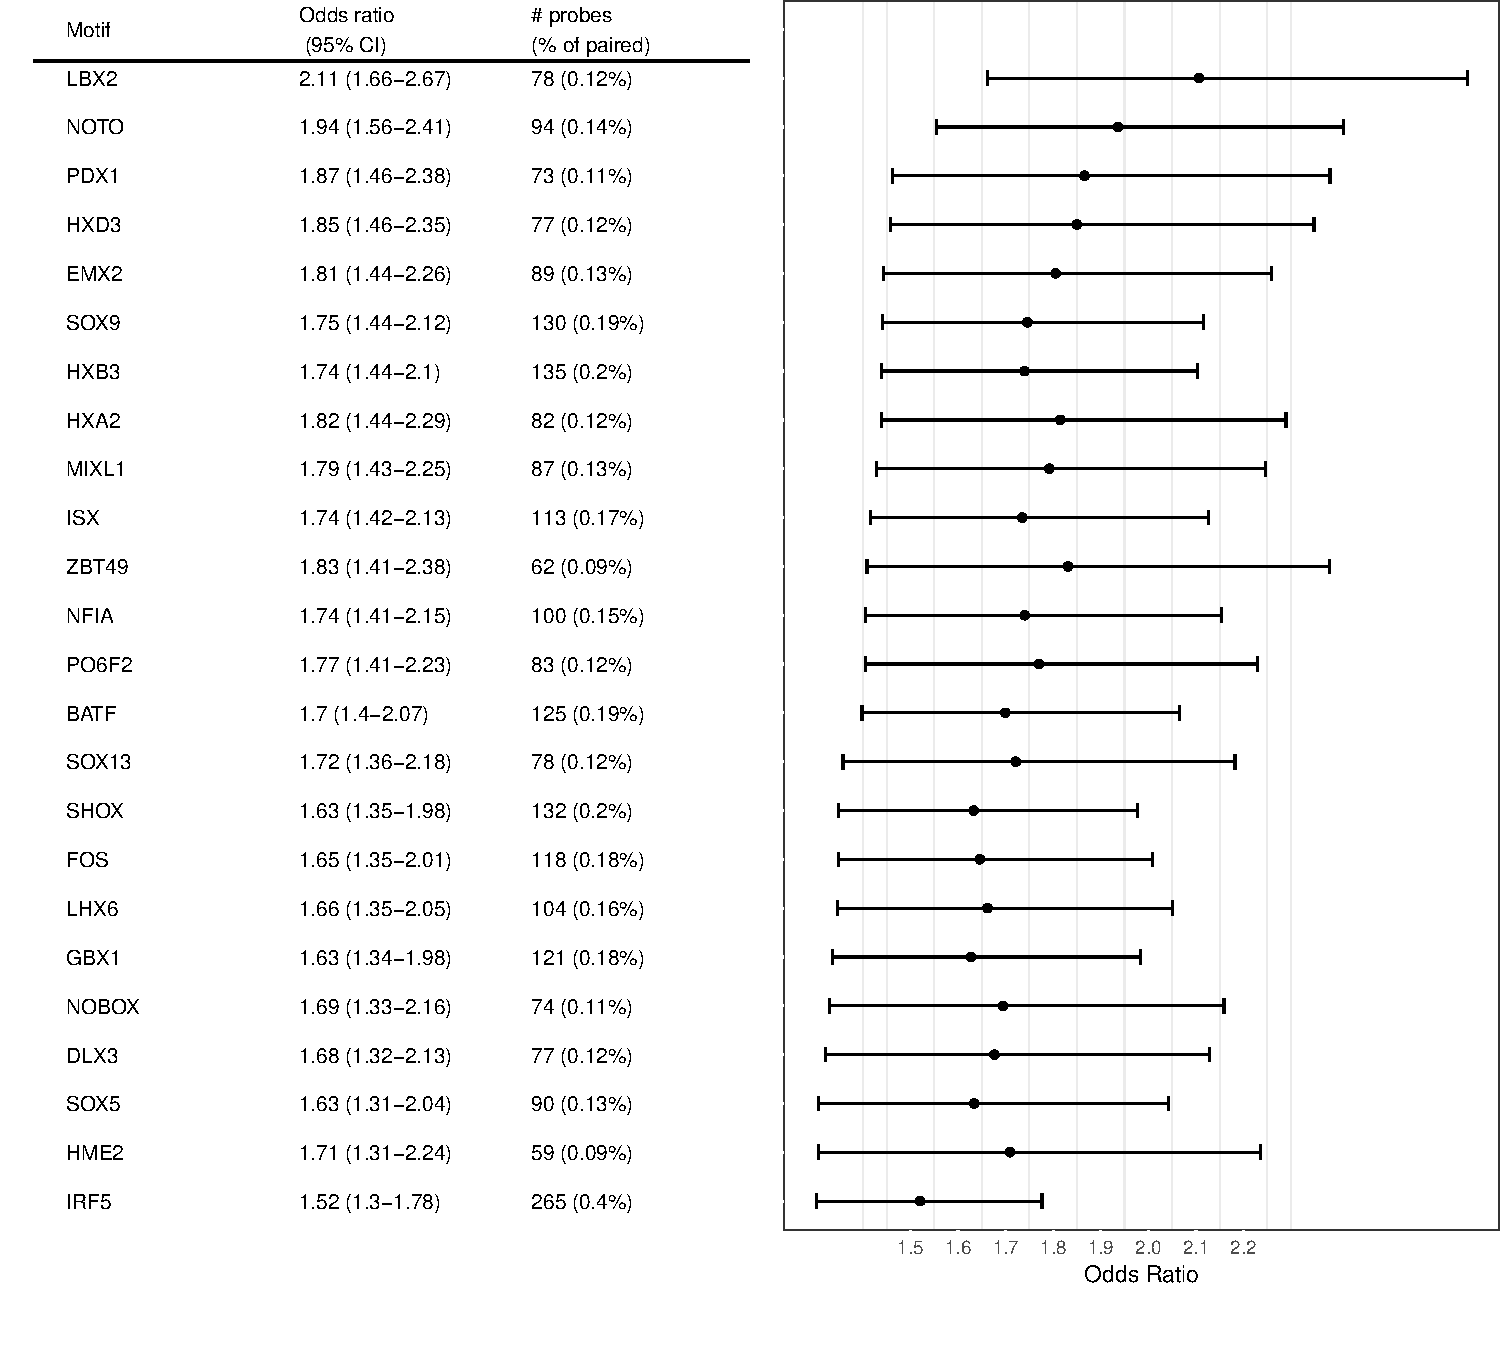
\includegraphics[width=16cm]{images/hyper_motif_enrichment.pdf}
\begin{flushleft}
\captionof{figure}{Motif enrichment analysis: Odds Ratio (x axis) for the selected motifs with OR above 1.5. The range shows the 95\% confidence interval for each Odds Ratio.}
\end{flushleft}
\end{figure}
\label{tab:or}
\end{center}


For example, in Table \ref{tab:tf} the motif HXD3 has as potential TF candidate the HOXD13 if we consider the family \sigla{TF}{Transcription Factor} classification and the HOXD3 TF candidate considering the subfamily TF classification. Figure \ref{tab:hocomoco} shows the motif signature for the HOX-related factors family from \sigla{HOCOMOCO}{HOmo sapiens COmprehensive MOdel COllection} database. The transcription factors \sigla{HOXD13}{Homeobox D13} and \sigla{HOXD3}{Homeobox D3} are in the same family (HOX-related factors) but in different subfamilies.



\begin{table}[h!]
\centering
\caption{TF ranking analysis: statistic For each enriched motif the anti-correlation level of all human TFs expression level with average DNA methylation level at sites with a given motif was access and ranked by the $-log_{10}(P_{value})$, the most relevant one that belongs to the same family as the motif is shown in column \textit{top.potential.TF.family} while the most relevant within the same sub-family classification is shown in column \textit{top.potential.TF.subfamily}}.
\csvautobooktabular[respect underscore]{tables/getTF.hyper.significant.TFs.with.motif.summary.csv}
\label{tab:tf}
\end{table}

\begin{center}
\begin{figure}[h!]
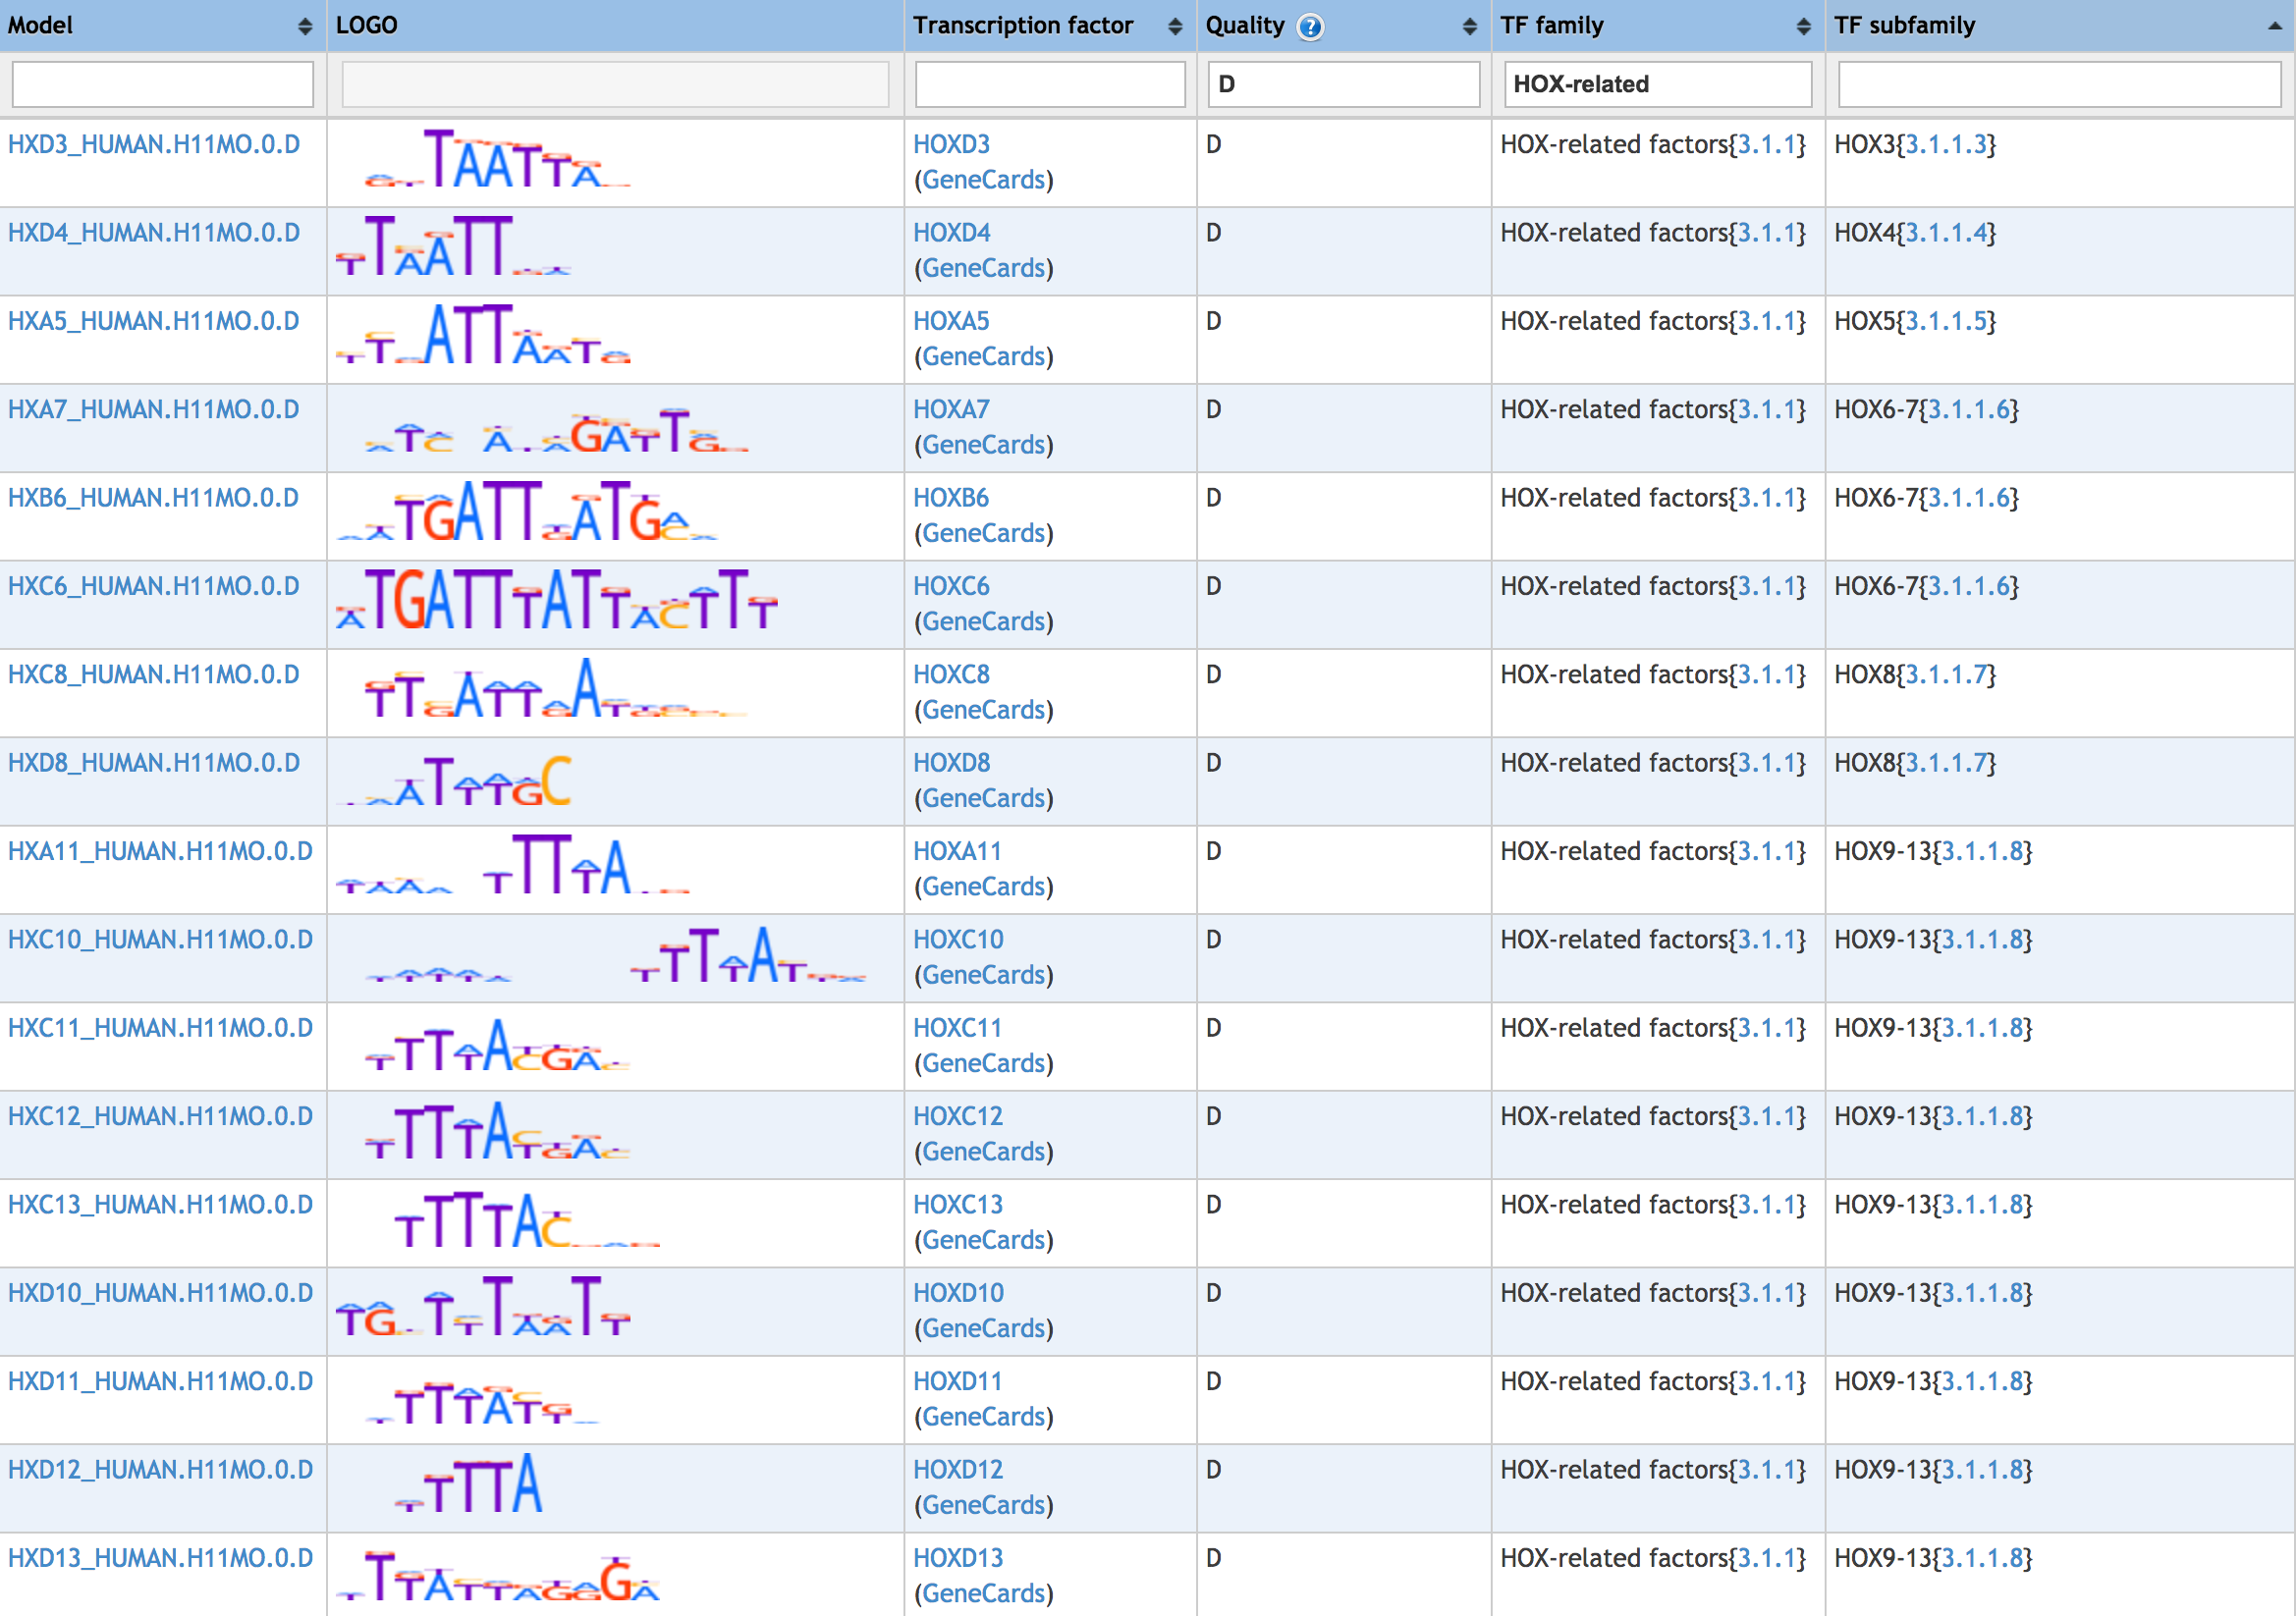
\includegraphics[width=16cm]{images/HOCOMOCO.png}
\caption{HOCOMOCO V11: HOX-related factors family. Transcription factors HOXD13 and HOXD3 are in the same family (HOX-related factors) but in different subfamilies.}
\end{figure}
\label{tab:hocomoco}
\end{center}

To validate those findings, biological experiments are needed which by either knocking down the TF or by regulating the DNA methylation levels of those binding regions will be able to verify if the downstream genes are being regulated.




\chapter{Citações e referências}
\label{chapter:citacoes}
Em documentos acadêmicos podem existir as citações podem ser: \textbf{implícitas} quando as referências não fazem parte do texto ou \textbf{explícitas} quando o autor referente a citação é mencionado explicitamente na sentença. Nesse sentido, deve-se utilizar os comandos específicos para cada tipo de citação, ou seja, em citações explicitas deve-se usar o comando \comando{citeonline\{\}} e nas demais situações é usado o comando \comando{cite\{\}}. Alguns exemplos são apresentados no \autoref{qua:exemplo-citacao}.

\begin{quadro}[htb]
\caption{Exemplos de citações no documento}
\label{qua:exemplo-citacao}
\centering\small 
\begin{tabular}{|c|c|}        \hline
\textbf{Código em \LaTeX} & \textbf{Código Compilado}\\ \hline\hline
\begin{minipage}[t]{\VerbL}
\vspace{5pt}
\begin{verbatim}
A ironia será assim uma ... proposta
por \citeonline{10520:2000:4.1-1}.
\end{verbatim}
\vspace{5pt}
\end{minipage}
&
\begin{minipage}[t]{\LatL}
\vspace{5pt}
A ironia será assim uma ... proposta 
por \citeonline{10520:2000:4.1-1}.
\vspace{5pt}
\end{minipage}\\\hline

\begin{minipage}[t]{\VerbL}
\vspace{5pt}
\begin{verbatim}
\citeonline[p.~146]{10520:2000:4.2-2}
dizem que ... 
\end{verbatim}
\vspace{5pt}
\end{minipage}
&
\begin{minipage}[t]{\LatL}
\vspace{5pt}
\citeonline[p.~146]{10520:2000:4.2-2} dizem que {...}
\vspace{5pt}
\end{minipage}\\ \hline

\begin{minipage}[t]{\VerbL}
\vspace{5pt}
\begin{verbatim}
``Apesar das ... da filosofia''
\cite[p.~293]{10520:2000:4.1-2}.
\end{verbatim}
\vspace{5pt}
\end{minipage}
&
\begin{minipage}[t]{\LatL}
\vspace{5pt}
``Apesar das {...} da filosofia'' \cite[p.~293]{10520:2000:4.1-2}.
\vspace{5pt}
\end{minipage} \\ \hline

\begin{minipage}[t]{\VerbL}
\vspace{5pt}
\begin{verbatim}
Depois, ...  que prefiro
\cite{10520:2000:4.1-3}.
\end{verbatim}
\vspace{5pt}
\end{minipage}
&
\begin{minipage}[t]{\LatL}
\vspace{5pt}
Depois, {...} que prefiro \cite{10520:2000:4.1-3}.
\vspace{5pt}
\end{minipage}\\ \hline

\end{tabular}
\end{quadro}


Para especificar a página, seção ou capítulo consultado na referência é preciso acrescentá-lo entre colchetes com os comandos \comando{cite[página]\{\}} ou \comando{citeonline[página]\{\}}. O texto colocado entre colchetes aparecerá logo após o ano. Maiores informações sobre os comandos utilizados para citação posem ser consultados no manual de referência da abnTeX2, incluindo o uso de \textbf{apud} \cite{abntex2cite-alf}.


\section{Citações Indiretas}

As citações indiretas são caracterizadas como uma espécie de paráfrase das ideias de um determinado autor, ou seja, o pesquisador, por meio de suas próprias palavras, interpreta o discurso de outrem, contudo, mantendo o mesmo sentido. Outro aspecto que deve ser considerado é a necessidade de o autor (ou os autores) e o ano em que a obra foi publicada serem mencionados. 

Nas citações indiretas há duas formatações possíveis dependendo de como ocorre a citação no texto. Quando o autor é mencionado explicitamente utiliza-se o comando \comando{citeonline\{\}}, caso contrário, deve utilizar o comando \comando{cite\{\}}. 



\section{Citações diretas}
\label{sec-citacao}


As citações diretas ocorrem quando o texto de uma referência é transcrito literalmente. As citações diretas curtas (até três linhas) são inseridas no texto entre aspas duplas. As aspas simples são utilizadas para indicar citação no interior da citação: \aspas{Nas citações, as chamadas pelo sobrenome do autor [...] incluído na sentença devem ser em letras maiúsculas e minúsculas e, quando estiverem entre parênteses, devem ser em letras maiúsculas} \cite[sec.~5]{NBR10520:2002}.

\begin{verbatim}
``Nas citações, as chamadas pelo sobrenome do autor [...] incluído na 
sentença devem ser em letras maiúsculas e minúsculas e, quando 
estiverem entre parênteses, devem ser em letras maiúsculas''
\cite[5]{NBR10520:2002}.
\end{verbatim}

Cabe ressaltar que em \LaTeX as aspas iniciais são diferentes das finais. Para tanto, pode-se utilizar o comando \comando{aspas\{CONTEUDO\}} para inserir um determinado conteúdo entre aspas.

As citações diretas longas (com mais de 3 linhas) podem ser inseridas por meio do ambiente \texttt{citacao}:

\begin{citacao}
As citações diretas, no texto, com mais de três linhas, devem ser
destacadas com recuo de 4 cm da margem esquerda, com letra menor que a do texto
utilizado e sem as aspas. No caso de documentos datilografados, deve-se
observar apenas o recuo \cite[5.3]{NBR10520:2002}.
\end{citacao}

Use o ambiente assim:

\begin{verbatim}
\begin{citacao}
As citações diretas, no texto, com mais de três linhas [...] deve-se 
observar apenas o recuo \cite[5.3]{NBR10520:2002}.
\end{citacao}
\end{verbatim}

O ambiente \texttt{citacao} pode receber como parâmetro opcional um nome de
idioma previamente carregado nas opções da classe (\autoref{sec-hifenizacao}). Nesse
caso, o texto da citação é automaticamente escrito em itálico e a hifenização é
ajustada para o idioma selecionado na opção do ambiente. Por exemplo:

\begin{verbatim}
\begin{citacao}[english]
Text in English language in italic with correct hyphenation.
\end{citacao}
\end{verbatim}

Tem como resultado:

\begin{citacao}[english]
Text in English language in italic with correct hyphenation.
\end{citacao}


% ---
% Finaliza a parte no bookmark do PDF, para que se inicie o bookmark na raiz
% ---
\bookmarksetup{startatroot}% 
% ---

% ----------------------------------------------------------
% ELEMENTOS PÓS-TEXTUAIS
% ----------------------------------------------------------
\postextual

% ----------------------------------------------------------
% Referências bibliográficas
% ----------------------------------------------------------
\bibliography{references}

% ---------------------------------------------------------------------
% GLOSSÁRIO
% ---------------------------------------------------------------------

% Arquivo que contém as definições que vão aparecer no glossário
\newword{WYSIWYG}{``What You See Is What You Get''  ou ``O que você vê é o que você obtém''.  Recurso tem por objetivo permitir que um documento, enquanto manipulado na tela, tenha a mesma aparência de sua utilização, usualmente sendo considerada final. Isso facilita para o desenvolvedor que pode trabalhar visualizando a aparência do documento sem precisar salvar em vários momentos e abrir em um \textit{software} separado de visualização}
\newword{Framework}{é uma abstração que une códigos comuns entre vários projetos de \textit{software} provendo uma funcionalidade genérica. \textit{Frameworks} são projetados com a intenção de facilitar o desenvolvimento de \textit{software}, habilitando designers e programadores a gastarem mais tempo determinando as exigências do \textit{software} do que com detalhes de baixo nível do sistema}

\newword{Template}{é um documento sem conteúdo, com apenas a apresentação visual (apenas cabeçalhos por exemplo) e instruções sobre onde e qual tipo de conteúdo deve entrar a cada parcela da apresentação}

\newword{Padrões de projeto}{ou \textit{Design Pattern}, descreve uma solução geral reutilizável para um problema recorrente no desenvolvimento de sistemas de \textit{software} orientados a objetos. Não é um código final, é uma descrição ou modelo de como resolver o problema do qual trata, que pode ser usada em muitas situações diferentes}

\newword{Web}{Sinônimo mais conhecido de \textit{World Wide Web} (WWW). É a interface gráfica da Internet que torna os serviços disponíveis totalmente transparentes para o usuário e ainda possibilita a manipulação multimídia da informação}
% Comando para incluir todas as definições do arquivo glossario.tex
\glsaddall
% Impressão do glossário
\printglossaries

% ----------------------------------------------------------
% Apêndices
% ----------------------------------------------------------

% ---
% Inicia os apêndices
% ---
\begin{apendicesenv}

    \chapter{Documento básico usando a classe \textit{icmc}}
    \label{chapter:documento-basico}
    \definecolor{gray}{rgb}{0.4,0.4,0.4}
\definecolor{darkblue}{rgb}{0.0,0.0,0.6}
\definecolor{cyan}{rgb}{0.0,0.6,0.6}
\definecolor{maroon}{rgb}{0.5,0,0}
\definecolor{darkgreen}{rgb}{0,0.5,0}


\lstdefinelanguage{myLatex}
{
    keywords={\titulo},
    alsoletter={-},
    sensitive=false,
    morecomment=[l]{\%},
    morecomment=[s]{/*}{*/},
    morestring=[b]",
    morestring=[b]',
    keywordstyle=\bfseries\color{blue},
    commentstyle=\itshape\color{darkgreen},
    morekeywords={documentclass, titulo, autor, data, orientador, coorientador, curso, textoresumo, incluifichacatalografica, textodedicatoria*, textoagradecimentos*, textoepigrafe*, incluilistadefiguras, incluilistadetabelas, incluilistadequadros, incluilistadealgoritmos, incluilistadecodigos, incluilistadesiglas, incluilistadesimbolos, textual, chapter, postextual, begin, bibliography, end}, 
alsoletter={*, \{, \}, \[, \]},
 morekeywords=[2]{\{, \}, \[, \]},
 keywordstyle=[2]\bfseries\color{blue},
 moredelim=[s][\color{maroon}]{\{}{\}},
    moredelim=[s][\itshape\color{maroon}]{\[}{\]},
}

%\lstdefinelanguage{TeX}
%{
%moredelim=*[s][\color{maroon}]{\{}{\}}
%otherkeywords={\{, \}, \[, \], \\}
%  morestring=[b]",
%  moredelim=[s][\bfseries\color{maroon}]{<}{\ },
%  moredelim=[s][\bfseries\color{maroon}]{</}{>},
%  moredelim=[l][\bfseries\color{maroon}]{/>},
%  moredelim=[l][\bfseries\color{maroon}]{>},
%  commentstyle=\color{darkgreen},
%  stringstyle=\color{blue},
%  identifierstyle=\color{red},
%  keywordstyle=\bfseries\color{maroon}
%moredelim=[l][\bfseries\color{maroon}]{>},
%commentstyle=\color{darkgreen},
%  stringstyle=\color{blue},
%  identifierstyle=\color{red}, moredelim=[l][\bfseries\color{maroon}]{\{},
%  keywordstyle=\bfseries\color{maroon}
%}

%\lstset{language={[LaTeX]TeX},
%texcsstyle=*\bfseries\color{blue},
%keywordstyle=\bfseries\color{blue},
%commentstyle=\color{darkgreen},
%morecomment=[s][\color{red}]{\{}{\}},
%otherkeywords={$, \{, \}, \[, \]}
%}

%\begin{codigo}[caption={Exemplo de um documento básico}, label={codigo:documento-basico}, language={[LaTeX]TeX},  breaklines=true,morekeywords={titulo, autor, data, orientador, coorientador, curso, textoresumo, incluifichacatalografica, textodedicatoria*, textoagradecimentos*, textoepigrafe*, incluilistadefiguras, incluilistadetabelas, incluilistadequadros, incluilistadealgoritmos, incluilistadecodigos, incluilistadesiglas, incluilistadesimbolos, {\backslash}textual, chapter, postextual}, alsoletter={{\backslash},*},morecomment=[s][\color{red}]{\{}{\}}]
\begin{codigo}[caption={Exemplo de um documento básico}, label={codigo:documento-basico}, language={myLatex},  breaklines=true]
% Documento utilizando a classe icmc
% Opções: 
%   Qualificação         = qualificacao 
%   Curso                = doutorado/mestrado
%   Situação do trabalho = pre-defesa/pos-defesa (exceto para qualificação)
% -- opções do pacote babel --
% Idioma padrão = brazil
	%spanish,			% idioma adicional para hifenização
	%english,			% idioma adicional para hifenização
	%brazil				% o último idioma é o principal do documento
\ documentclass[doutorado, spanish, english, brazil]{packages/icmc}

% Título do trabalho
\titulo{Título da Monografia}

% Nome do autor
\autor[Abreviação]{Nome completo do autor}

% Data do depósito
\data{18}{12}{2012}

% Nome do Orientador
\orientador[Orientador]{Titulação do orientador}{Nome completo do Orientador}

% Nome do Coorientador (caso não exista basta remover)
\coorientador[Coorientador]{Titulação do coorientador}{Nome completo do Coorientador}
% Se coorientadora troque Coorientador: por Coorientadora dentro do colchetes

% Sigla do programa de Pós-graduação (CCMC, MAT, PIPGES, PROFMAT, MECAI)
\curso{CCMC}
% O valor entre colchetes é opcional para este programa

% Resumo
\textoresumo[Idioma]{
Texto do resumo do trabalho.
}{Lista de palavras-chave separada por virgulas}

% ----------------------------------------------------------
% ELEMENTOS PRÉ-TEXTUAIS
% ----------------------------------------------------------

% Inserir a ficha catalográfica
\incluifichacatalografica{634} % Código Cutter: número atribuído ao sobrenome do autor (disponível em http://www.davignon.qc.ca/cutter1.html).

% Incluí o texto da Dedicatória
\textodedicatoria*{tex/pre-textual/dedicatoria}

% Incluí o texto dos Agradecimentos
\textoagradecimentos*{tex/pre-textual/agradecimentos}

% Incluí o texto da Epígrafe
\textoepigrafe*{tex/pre-textual/epigrafe}

% Inclui a lista de figuras
\incluilistadefiguras

% Inclui a lista de tabelas
\incluilistadetabelas

% Inclui a lista de quadros
\incluilistadequadros

% Inclui a lista de algoritmos
\incluilistadealgoritmos

% Inclui a lista de códigos
\incluilistadecodigos

% Inclui a lista de siglas e abreviaturas
\incluilistadesiglas

% Inclui a lista de símbolos
\incluilistadesimbolos

% Início do documento
\begin{document}

% ----------------------------------------------------------
% ELEMENTOS TEXTUAIS
% ----------------------------------------------------------
\textual

\chapter{Introdução}

Capítulo de Introdução

\chapter{Desenvolvimento}

Capítulo de Desenvolvimento

\chapter{Conclusão}

Capítulo de conclusão

% ----------------------------------------------------------
% ELEMENTOS PÓS-TEXTUAIS
% ----------------------------------------------------------
\postextual

% Nome do arquivo com as referências bibliográficas
\bibliography{referencias}

\end{document}

\end{codigo}
    
    \chapter{Configuração do programa JabRef}
    \label{chapter:configuracao-jabref}
    \lstdefinelanguage{XML}
{
  morestring=[b]",
  moredelim=[s][\bfseries\color{maroon}]{<}{\ },
  moredelim=[s][\bfseries\color{maroon}]{</}{>},
  moredelim=[l][\bfseries\color{maroon}]{/>},
  moredelim=[l][\bfseries\color{maroon}]{>},
  morecomment=[s]{<?}{?>},
  morecomment=[s]{<!--}{-->},
  commentstyle=\color{darkgreen},
  stringstyle=\color{blue},
  identifierstyle=\color{red}
}


\begin{codigo}[caption={Código de configuração do programa JabRef em XML}, label={codigo:config-jabref}, language=XML, breaklines=true]
<?xml version="1.0" encoding="UTF-8" standalone="no"?>
<!DOCTYPE preferences SYSTEM "http://java.sun.com/dtd/preferences.dtd">
<preferences EXTERNAL_XML_VERSION="1.0">
  <root type="user">
    <map/>
    <node name="net">
      <map/>
      <node name="sf">
        <map/>
        <node name="jabref">
          <map>
            <entry key="KeyPatternRegex" value=""/>
            <entry key="KeyPatternReplacement" value=""/>
            <entry key="abbrAuthorNames" value="true"/>
            <entry key="allowTableEditing" value="false"/>
            <entry key="autoComplete" value="true"/>
            <entry key="autoCompleteFields" value="author;editor;title;journal;publisher;keywords;crossref"/>
            <entry key="autoDoubleBraces" value="true"/>
            <entry key="autoOpenForm" value="true"/>
            <entry key="autoResizeMode" value="4"/>
            <entry key="autoSave" value="true"/>
            <entry key="autoSaveInterval" value="5"/>
            <entry key="autolinkExactKeyOnly" value="true"/>
            <entry key="avoidOverwritingKey" value="false"/>
            <entry key="backup" value="false"/>
            <entry key="caseSensitiveSearch" value="false"/>
            <entry key="citeseerColumn" value="false"/>
            <entry key="confirmDelete" value="true"/>
            <entry key="ctrlClick" value="false"/>
            <entry key="customTypeName_0" value="Article"/>
            <entry key="customTypeName_1" value="Book"/>
            <entry key="customTypeName_10" value="Misc"/>
            <entry key="customTypeName_11" value="Monography"/>
            <entry key="customTypeName_12" value="Patent"/>
            <entry key="customTypeName_13" value="Periodical"/>
            <entry key="customTypeName_14" value="Phdthesis"/>
            <entry key="customTypeName_15" value="Proceedings"/>
            <entry key="customTypeName_16" value="Standard"/>
            <entry key="customTypeName_17" value="Techreport"/>
            <entry key="customTypeName_2" value="Booklet"/>
            <entry key="customTypeName_3" value="Conference"/>
            <entry key="customTypeName_4" value="Electronic"/>
            <entry key="customTypeName_5" value="Inbook"/>
            <entry key="customTypeName_6" value="Incollection"/>
            <entry key="customTypeName_7" value="Inproceedings"/>
            <entry key="customTypeName_8" value="Manual"/>
            <entry key="customTypeName_9" value="Mastersthesis"/>
            <entry key="customTypeOpt_0" value="month;part;section;url;urlaccessdate;note"/>
            <entry key="customTypeOpt_1" value="subtitle;edition;pages;number;series;isbn;volume;org-short;url;urlaccessdate;note"/>
            <entry key="customTypeOpt_10" value="howpublished;month;year;publisher;subtitle;pages;pagename;address;series;number;editortype;url;urlaccessdate;note"/>
            <entry key="customTypeOpt_11" value="pages;pagename;url;urlaccessdate;note"/>
            <entry key="customTypeOpt_12" value="author;title;language;assignee;address;type;number;day;dayfiled;month;monthfiled;url;note"/>
            <entry key="customTypeOpt_13" value="editor;language;series;volume;number;organization;month;url;org-short;note"/>
            <entry key="customTypeOpt_14" value="pages;pagename;url;urlaccessdate;note"/>
            <entry key="customTypeOpt_15" value="editor;volume;number;series;address;publisher;month;organization;org-short;note"/>
            <entry key="customTypeOpt_16" value="author;language;howpublished;type;number;revision;address;month;year;url;org-short;note"/>
            <entry key="customTypeOpt_17" value="pages;pagename;org-short;url;urlaccessdate;number;month;note"/>
            <entry key="customTypeOpt_2" value="subtitle;edition;pages;number;volume;org-short;url;urlaccessdate;note"/>
            <entry key="customTypeOpt_3" value="editor;volume;number;series;pages;address;month;organization;publisher;org-short;note"/>
            <entry key="customTypeOpt_4" value="month;year;org-short;note"/>
            <entry key="customTypeOpt_5" value="booksubtitle;edition;number;series;isbn;volume;org-short;editortype;url;urlaccessdate;note"/>
            <entry key="customTypeOpt_6" value="booksubtitle;edition;number;series;isbn;volume;org-short;editortype;url;urlaccessdate;note"/>
            <entry key="customTypeOpt_7" value="pages;month;publisher;booktitle;conference-location;conference-year;url;urlaccessdate;note"/>
            <entry key="customTypeOpt_8" value="subtitle;author;organization;org-short;address;edition;month;year;pages;series;url;urlaccessdate;note"/>
            <entry key="customTypeOpt_9" value="pages;pagename;url;urlaccessdate;note"/>
            <entry key="customTypeReq_0" value="author;title;journal;year;volume;number;pages"/>
            <entry key="customTypeReq_1" value="title;author/editor/organization;publisher;year;address"/>
            <entry key="customTypeReq_10" value=";author/organization/editor/title"/>
            <entry key="customTypeReq_11" value="author;title;type;school;year;address"/>
            <entry key="customTypeReq_12" value="nationality;number;year;yearfiled"/>
            <entry key="customTypeReq_13" value="title;year"/>
            <entry key="customTypeReq_14" value="author;title;school;year;address"/>
            <entry key="customTypeReq_15" value="title;year"/>
            <entry key="customTypeReq_16" value="title;organization/institution"/>
            <entry key="customTypeReq_17" value="author;title;organization/school;year;address"/>
            <entry key="customTypeReq_2" value="title;author/editor/organization;year"/>
            <entry key="customTypeReq_3" value="author;title;booktitle;year"/>
            <entry key="customTypeReq_4" value="url;urlaccessdate;author/organization/title"/>
            <entry key="customTypeReq_5" value="author;title;editor/organization;booktitle;chapter/pages;publisher;address;year"/>
            <entry key="customTypeReq_6" value="author;title;booktitle;editor/organization;chapter/pages;publisher;address;year"/>
            <entry key="customTypeReq_7" value="author;title;organization;conference-number;year;address"/>
            <entry key="customTypeReq_8" value="title"/>
            <entry key="customTypeReq_9" value="author;title;school;year;address"/>
            <entry key="defaultEncoding" value="ISO8859_15"/>
            <entry key="defaultLabelPattern" value="[auth]:[year]"/>
            <entry key="defaultOwner" value=""/>
            <entry key="defaultShowSource" value="false"/>
            <entry key="dialogWarningForDuplicateKey" value="true"/>
            <entry key="dialogWarningForEmptyKey" value="true"/>
            <entry key="disableOnMultipleSelection" value="false"/>
            <entry key="doNotResolveStringsFor" value="url"/>
            <entry key="enableSourceEditing" value="true"/>
            <entry key="enforceLegalBibtexKey" value="true"/>
            <entry key="exportInOriginalOrder" value="false"/>
            <entry key="exportInStandardOrder" value="true"/>
            <entry key="exportWorkingDirectory" value="/home/marcos/tmp"/>
            <entry key="fileColumn" value="true"/>
            <entry key="fileDirectory" value=""/>
            <entry key="filechooserDisableRename" value="true"/>
            <entry key="floatMarkedEntries" value="true"/>
            <entry key="floatSearch" value="true"/>
            <entry key="fontFamily" value="SansSerif"/>
            <entry key="fontSize" value="12"/>
            <entry key="fontStyle" value="0"/>
            <entry key="generateKeysAfterInspection" value="true"/>
            <entry key="generateKeysBeforeSaving" value="false"/>
            <entry key="gridColor" value="210:210:210"/>
            <entry key="groupAutoHide" value="true"/>
            <entry key="groupAutoShow" value="true"/>
            <entry key="groupExpandTree" value="true"/>
            <entry key="groupKeywordSeparator" value=", "/>
            <entry key="groupShowDynamic" value="true"/>
            <entry key="groupShowIcons" value="true"/>
            <entry key="groupsDefaultField" value="keywords"/>
            <entry key="incompleteEntryBackground" value="250:175:175"/>
            <entry key="incrementS" value="false"/>
            <entry key="lastEdited" value="/home/marcos/Documentos/IFMG/Acadêmico/Aulas/Latex/ifmgbitex/referencias.bib"/>
            <entry key="lastUsedExport" value="html"/>
            <entry key="lookAndFeel" value="com.jgoodies.plaf.plastic.Plastic3DLookAndFeel"/>
            <entry key="markImportedEntries" value="true"/>
            <entry key="markedEntryBackground" value="255:255:180"/>
            <entry key="memoryStickMode" value="false"/>
            <entry key="namesAsIs" value="false"/>
            <entry key="namesFf" value="false"/>
            <entry key="namesLastOnly" value="false"/>
            <entry key="namesNatbib" value="true"/>
            <entry key="openLastEdited" value="true"/>
            <entry key="overrideDefaultFonts" value="false"/>
            <entry key="overwriteOwner" value="false"/>
            <entry key="overwriteTimeStamp" value="false"/>
            <entry key="pdfColumn" value="false"/>
            <entry key="pdfDirectory" value=""/>
            <entry key="posX" value="0"/>
            <entry key="posY" value="0"/>
            <entry key="preview0" value="&lt;font face=&quot;arial&quot;&gt;&lt;b&gt;&lt;i&gt;\bibtextype&lt;/i&gt;&lt;a name=&quot;\bibtexkey&quot;&gt;\begin{bibtexkey} (\bibtexkey)&lt;/a&gt;\end{bibtexkey}&lt;/b&gt;&lt;br&gt;__NEWLINE__\begin{author} \format[HTMLChars,AuthorAbbreviator,AuthorAndsReplacer]{\author}&lt;BR&gt;\end{author}__NEWLINE__\begin{editor} \format[HTMLChars,AuthorAbbreviator,AuthorAndsReplacer]{\editor} &lt;i&gt;(\format[IfPlural(Eds.,Ed.)]{\editor})&lt;/i&gt;&lt;BR&gt;\end{editor}__NEWLINE__\begin{title} \format[HTMLChars]{\title} \end{title}&lt;BR&gt;__NEWLINE__\begin{chapter} \format[HTMLChars]{\chapter}&lt;BR&gt;\end{chapter}__NEWLINE__\begin{journal} &lt;em&gt;\format[HTMLChars]{\journal}, &lt;/em&gt;\end{journal}__NEWLINE__\begin{booktitle} &lt;em&gt;\format[HTMLChars]{\booktitle}, &lt;/em&gt;\end{booktitle}__NEWLINE__\begin{school} &lt;em&gt;\format[HTMLChars]{\school}, &lt;/em&gt;\end{school}__NEWLINE__\begin{institution} &lt;em&gt;\format[HTMLChars]{\institution}, &lt;/em&gt;\end{institution}__NEWLINE__\begin{publisher} &lt;em&gt;\format[HTMLChars]{\publisher}, &lt;/em&gt;\end{publisher}__NEWLINE__\begin{year}&lt;b&gt;\year&lt;/b&gt;\end{year}\begin{volume}&lt;i&gt;, \volume&lt;/i&gt;\end{volume}\begin{pages}, \format[FormatPagesForHTML]{\pages} \end{pages}__NEWLINE__\begin{abstract}&lt;BR&gt;&lt;BR&gt;&lt;b&gt;Abstract: &lt;/b&gt; \format[HTMLChars]{\abstract} \end{abstract}__NEWLINE__\begin{review}&lt;BR&gt;&lt;BR&gt;&lt;b&gt;Review: &lt;/b&gt; \format[HTMLChars]{\review} \end{review}&lt;/dd&gt;__NEWLINE__&lt;p&gt;&lt;/p&gt;&lt;/font&gt;"/>
            <entry key="preview1" value="&lt;font face=&quot;arial&quot;&gt;&lt;b&gt;&lt;i&gt;\bibtextype&lt;/i&gt;&lt;a name=&quot;\bibtexkey&quot;&gt;\begin{bibtexkey} (\bibtexkey)&lt;/a&gt;\end{bibtexkey}&lt;/b&gt;&lt;br&gt;__NEWLINE__\begin{author} \format[HTMLChars,AuthorAbbreviator,AuthorAndsReplacer]{\author}&lt;BR&gt;\end{author}__NEWLINE__\begin{editor} \format[HTMLChars,AuthorAbbreviator,AuthorAndsReplacer]{\editor} &lt;i&gt;(\format[IfPlural(Eds.,Ed.)]{\editor})&lt;/i&gt;&lt;BR&gt;\end{editor}__NEWLINE__\begin{title} \format[HTMLChars]{\title} \end{title}&lt;BR&gt;__NEWLINE__\begin{chapter} \format[HTMLChars]{\chapter}&lt;BR&gt;\end{chapter}__NEWLINE__\begin{journal} &lt;em&gt;\format[HTMLChars]{\journal}, &lt;/em&gt;\end{journal}__NEWLINE__\begin{booktitle} &lt;em&gt;\format[HTMLChars]{\booktitle}, &lt;/em&gt;\end{booktitle}__NEWLINE__\begin{school} &lt;em&gt;\format[HTMLChars]{\school}, &lt;/em&gt;\end{school}__NEWLINE__\begin{institution} &lt;em&gt;\format[HTMLChars]{\institution}, &lt;/em&gt;\end{institution}__NEWLINE__\begin{publisher} &lt;em&gt;\format[HTMLChars]{\publisher}, &lt;/em&gt;\end{publisher}__NEWLINE__\begin{year}&lt;b&gt;\year&lt;/b&gt;\end{year}\begin{volume}&lt;i&gt;, \volume&lt;/i&gt;\end{volume}\begin{pages}, \format[FormatPagesForHTML]{\pages} \end{pages}&lt;/dd&gt;__NEWLINE__&lt;p&gt;&lt;/p&gt;&lt;/font&gt;"/>
            <entry key="priDescending" value="false"/>
            <entry key="priSort" value="entrytype"/>
            <entry key="promptBeforeUsingAutosave" value="true"/>
            <entry key="psDirectory" value=""/>
            <entry key="pushToApplication" value="Insert selected citations into LyX/Kile"/>
            <entry key="recentFiles" value="/home/marcos/Documentos/IFMG/Acadêmico/Aulas/Algoritmos/Algoritmos_exercicios_01/referencias.bib;/home/marcos/Documentos/IFMG/TCC e Projetos/ERP Comparativo/referencias.bib"/>
            <entry key="regExpSearch" value="true"/>
            <entry key="rememberWindowLocation" value="true"/>
            <entry key="resolveStringsAllFields" value="false"/>
            <entry key="runAutomaticFileSearch" value="false"/>
            <entry key="saveInOriginalOrder" value="false"/>
            <entry key="saveInStandardOrder" value="true"/>
            <entry key="searchAll" value="false"/>
            <entry key="searchAllBases" value="false"/>
            <entry key="searchGen" value="true"/>
            <entry key="searchOpt" value="true"/>
            <entry key="searchPanelVisible" value="false"/>
            <entry key="searchReq" value="true"/>
            <entry key="secDescending" value="false"/>
            <entry key="secSort" value=""/>
            <entry key="selectS" value="false"/>
            <entry key="showSearchInDialog" value="false"/>
            <entry key="showSource" value="true"/>
            <entry key="sizeX" value="1280"/>
            <entry key="sizeY" value="800"/>
            <entry key="stringsPosX" value="340"/>
            <entry key="stringsPosY" value="200"/>
            <entry key="stringsSizeX" value="600"/>
            <entry key="stringsSizeY" value="400"/>
            <entry key="tableBackground" value="255:255:255"/>
            <entry key="tableColorCodesOn" value="true"/>
            <entry key="tableOptFieldBackground" value="230:255:230"/>
            <entry key="tableReqFieldBackground" value="230:235:255"/>
            <entry key="tableText" value="0:0:0"/>
            <entry key="terDescending" value="false"/>
            <entry key="terSort" value=""/>
            <entry key="timeStampField" value="timestamp"/>
            <entry key="timeStampFormat" value="dd/MM/yyyy"/>
            <entry key="unmarkAllEntriesBeforeImporting" value="true"/>
            <entry key="urlColumn" value="true"/>
            <entry key="useDefaultLookAndFeel" value="true"/>
            <entry key="useIEEEAbrv" value="true"/>
            <entry key="useImportInspectionDialog" value="true"/>
            <entry key="useImportInspectionDialogForSingle" value="true"/>
            <entry key="useNativeFileDialogOnMac" value="false"/>
            <entry key="useOwner" value="false"/>
            <entry key="useRegExpSearch" value="false"/>
            <entry key="useRemoteServer" value="false"/>
            <entry key="useTimeStamp" value="true"/>
            <entry key="useXmpPrivacyFilter" value="false"/>
            <entry key="warnAboutDuplicatesInInspection" value="true"/>
            <entry key="warnBeforeOverwritingKey" value="true"/>
            <entry key="windowMaximised" value="false"/>
            <entry key="workingDirectory" value="/home/marcos/Documentos/IFMG/Acadêmico/Aulas/Algoritmos/Algoritmos_exercicios_01"/>
          </map>
          <node name="labelPattern">
            <map/>
          </node>
        </node>
      </node>
    </node>
  </root>
</preferences>

\end{codigo}

\end{apendicesenv}
% ---


% ----------------------------------------------------------
% Anexos
% ----------------------------------------------------------

% ---
% Inicia os anexos
% ---
\begin{anexosenv}

    \chapter{Páginas interessantes na Internet} 
    \label{chapter:paginas-interessantes}
    \begin{description}
 \item[\url{http://www.tex-br.org}] Página em português com diversos tutoriais e referências interessantes sobre \LaTeX;
 \item[\url{http://en.wikibooks.org/wiki/LaTeX}] Livro em formato \textit{wiki} gratuito sobre \LaTeX;
 \item[\url{http://tobi.oetiker.ch/lshort/lshort.pdf}] Ótimo tutorial sobre \LaTeX (possui versão em português \url{http://alfarrabio.di.uminho.pt/~albie/lshort/ptlshort.pdf}, mas a versão em inglês é a mais atual);
 \item[\url{http://code.google.com/p/abntex2/}] Página do abnTeX2, grupo que desenvolve os pacotes e classes em \LaTeX para as normas da ABNT, nos quais a classe \textit{icmc} foi baseada;
\item[\url{http://www.more.ufsc.br}] Página do Mecanismo On-line para Referências  (MORE) desenvolvido pela UFSC;
\item[\url{http://detexify.kirelabs.org/classify.html}] Página para recuperar o código de símbolos em \LaTeX a partir do desenho fornecido pelo usuário.
 \end{description}

\end{anexosenv}
% ---

\end{document}